
%使用XeLaTeX编译
%版权所有,翻版必究
%本文件由程序自动生成,任何修改将被覆盖
%2019 年 01 月 23 日




%\FloatBarrier
\cleardoublepage
\chapter{
Qt Quick入门导引
}\label{c000010}





%......

%使用xelatex编译
%版权所有,翻版必究
%本文件由程序自动生成,任何修改将被覆盖





\section{
搭建开发环境
}\label{s100110}




%......


%使用XeLaTeX编译
%版权所有,翻版必究
%本文件由程序自动生成,任何修改将被覆盖
%2019 年 01 月 23 日




%

\FloatBarrier
\subsection{
在Windows平台下搭建开发环境
}\label{s000110}


\FloatBarrier
\subsubsection{
在Windows平台下安装Qt
}\label{ss000110}


读者可以到 \url{http://download.qt.io/archive/
}
下载最新的Qt运行环境。
然而,遗憾的是,从Qt 5.12.0开始从此网址下载的Windows平台下的Qt开发环境并不完整。
%介绍如何下载在线安装包...
读者不得不访问Qt官网 \url{https://www.qt.io
},
注册Qt帐号,然后按照流程下载在线安装包。
不得不说,这对初学者很不友好。
幸运的是,目前Qt网站有一个漏洞。读者可以直接访问
 \url{https://www.qt.io/download-thank-you
},点击“here”下载在线安装包。如\figurename\ \ref{p000000}。
%begin图片
\begin{figure}[htb] %浮动体 here and top ...
%there must use marginnote ...
\marginnote{\setlength\fboxsep{2pt}\fbox{\footnotesize{\kaishu\figurename\,}\footnotesize{\ref{p000000}}}}\centering %中心对齐
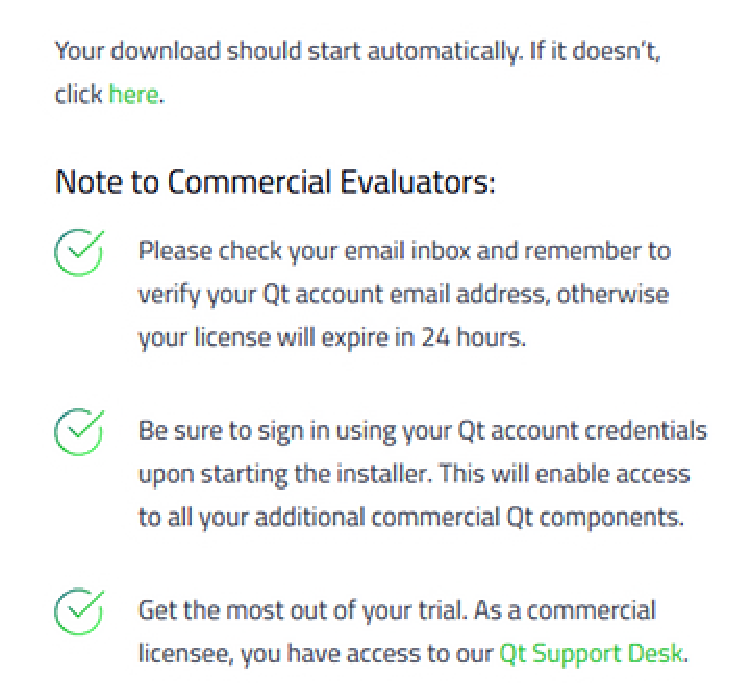
\includegraphics[width=8cm]{the_book_image/p000000.eps} %图片路径
\caption{Qt在线安装包下载路径} %标题
\label{p000000} %索引
\end{figure}
%end图片

以管理员身份运行在线安装包,
选择安装路径时请不要选择包含空格和中文字符的路径。
虽然现代开发环境对于空格和中文字符支持良好,
但是,很多第三方辅助工具未必支持空格和中文字符。
包括本书自带的辅助工具也不保证支持空格和中文。

在Windows平台下,建议读者选择安装“MSVC 2017 64\hspace{0.05em}\rule[0.7ex]{0.4em}{0.65pt}\hspace{0.05em}bit”或以上版
或者
“MinGW 7.3.0 64\hspace{0.05em}\rule[0.7ex]{0.4em}{0.65pt}\hspace{0.05em}bit”或以上版本。
Qt选择5.12.0或以上版本。
安装的时候最好选择安装“Sources”、“Qt Charts”、“Qt WebEngine”以及
“Qt Debug Information Files”这些模块。
在“Tools”选项下组好安装“CDB”以及对应的“MinGW”。
本书建议最小安装如\figurename\ \ref{p000001}。
%begin图片
\begin{figure}[htb] %浮动体 here and top ...
%there must use marginnote ...
\marginnote{\setlength\fboxsep{2pt}\fbox{\footnotesize{\kaishu\figurename\,}\footnotesize{\ref{p000001}}}}\centering %中心对齐
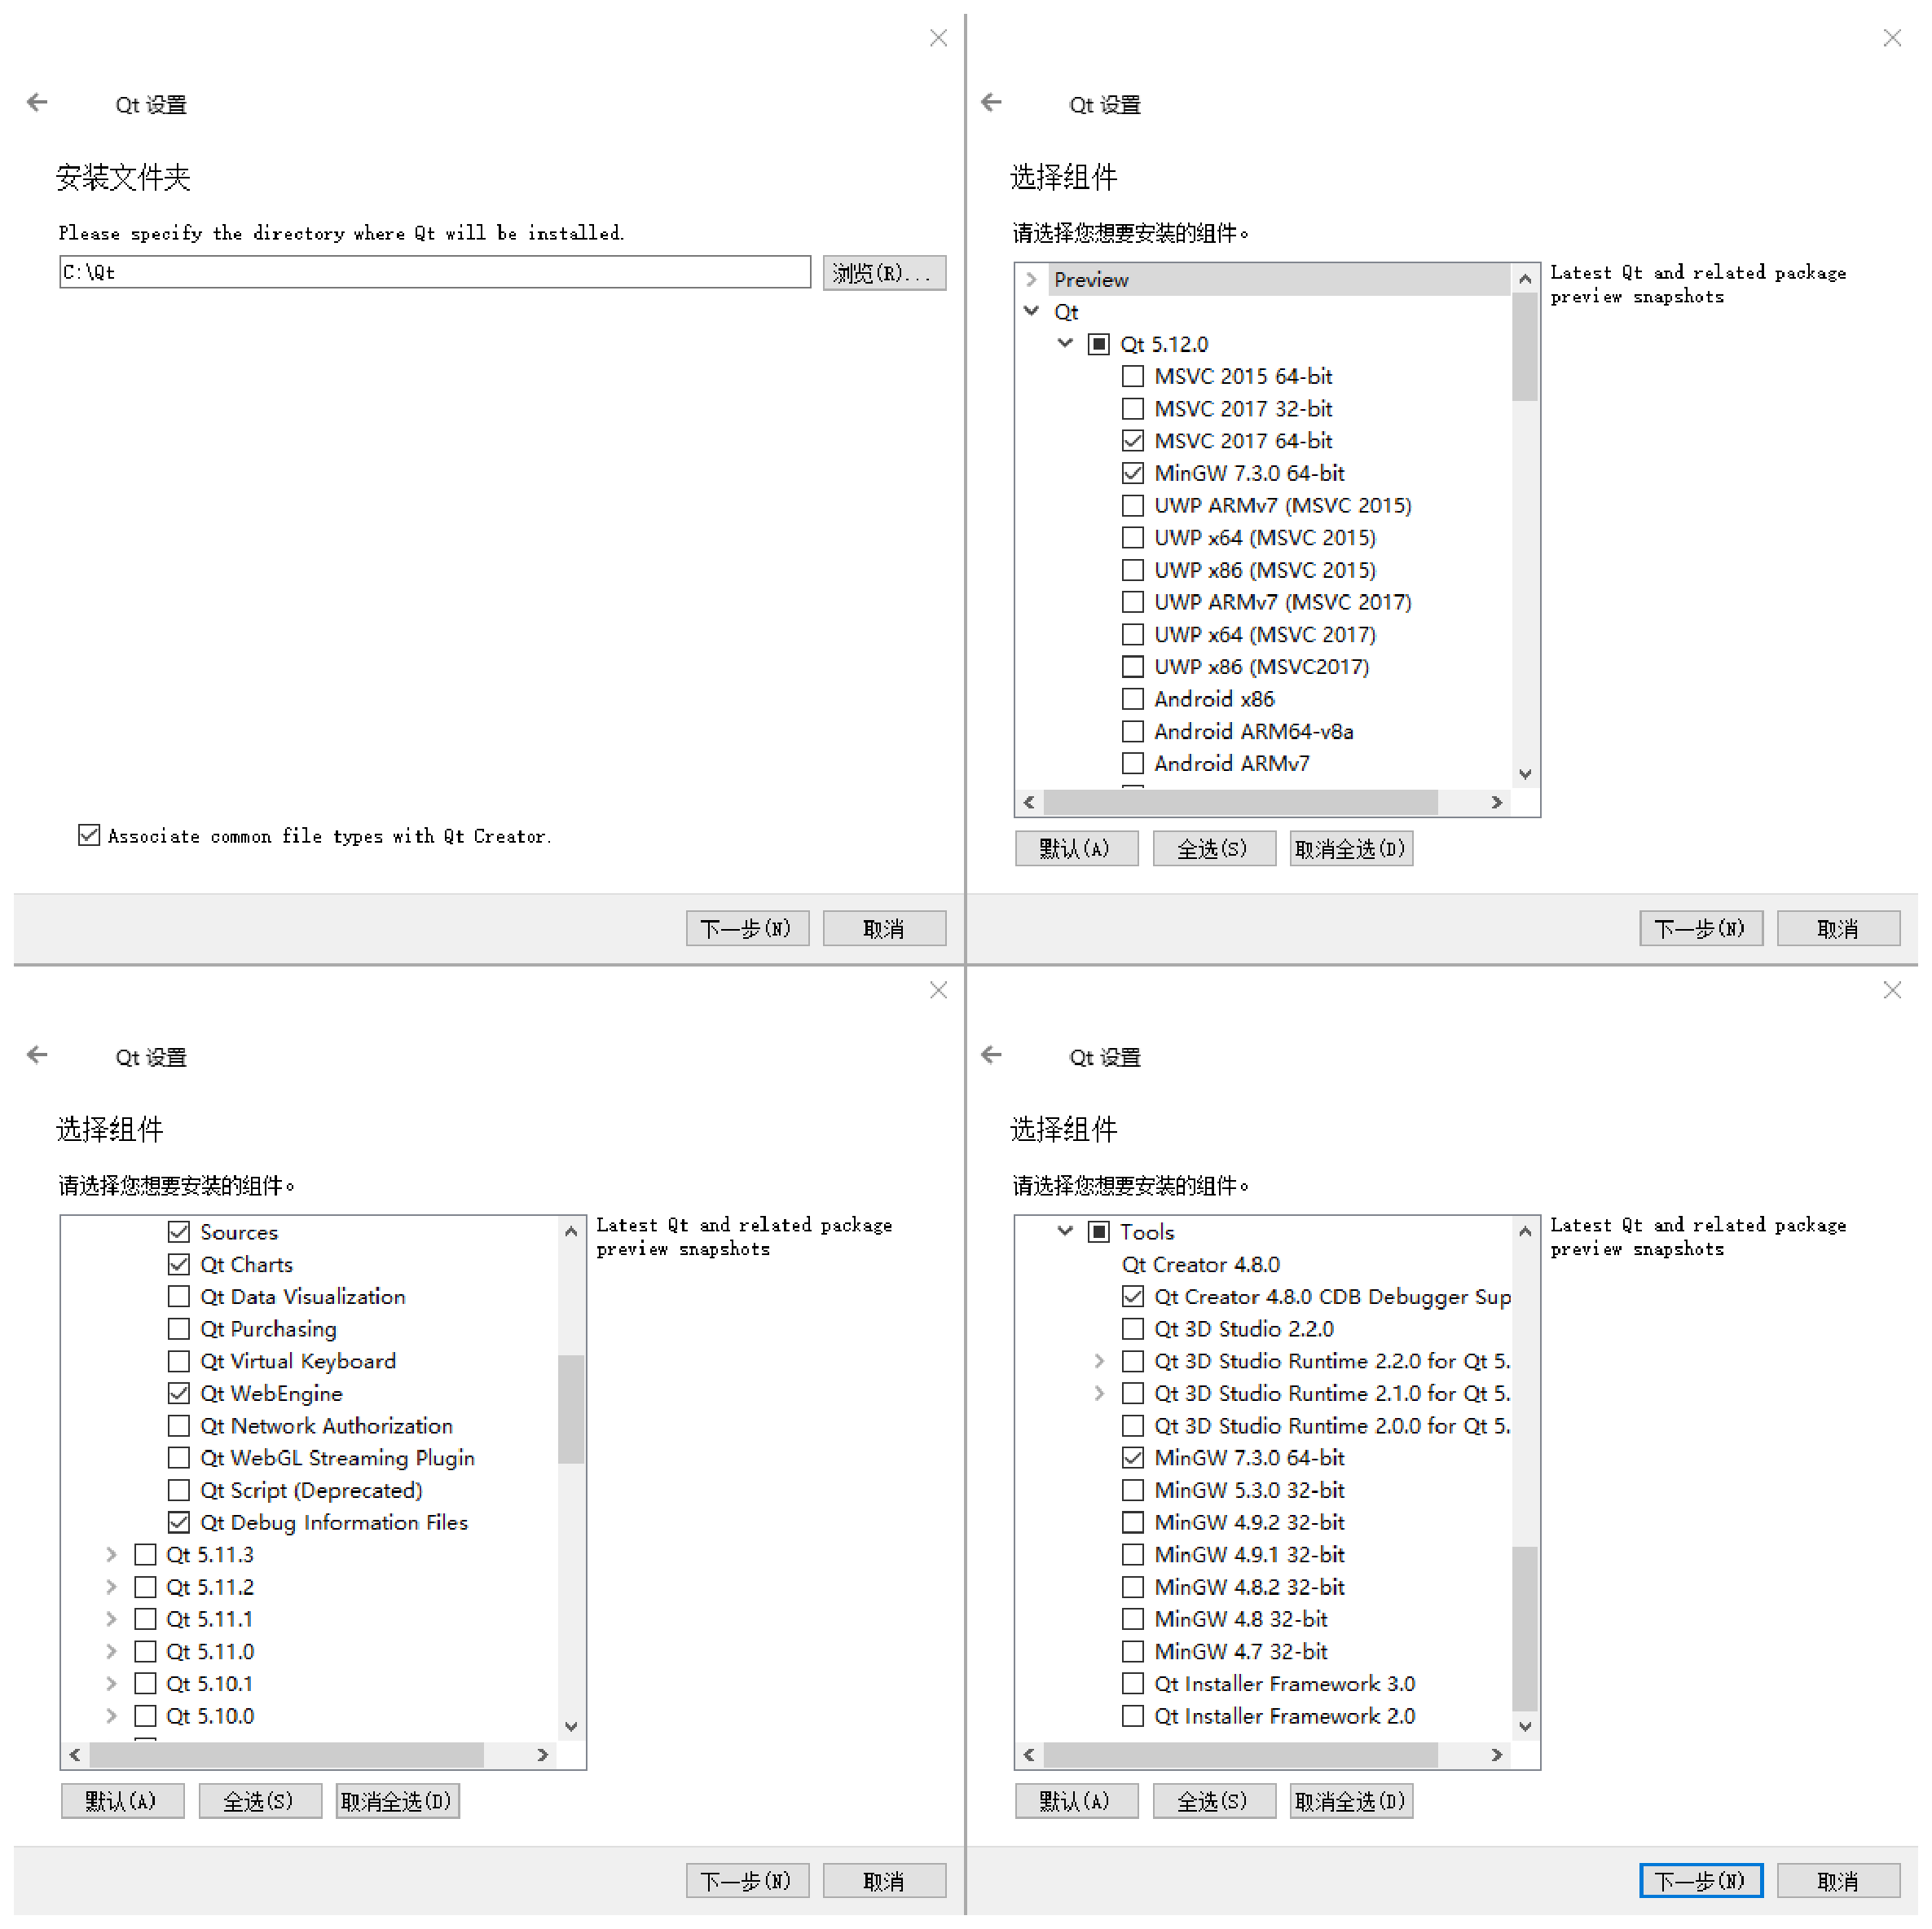
\includegraphics[width=0.95\textwidth]{the_book_image/p000001.eps} %图片路径
\caption{Qt在线安装建议安装组件} %标题
\label{p000001} %索引
\end{figure}
%end图片


\FloatBarrier
\subsubsection{
在Windows平台下安装Boost
}\label{ss000210}

读者需要到Boost官网 \url{https://www.boost.org/
}下载最新Boost稳定版。解压缩,将“boost”文件夹复制到Qt Include路径。

比如,
用户的Qt Include路径为:
\begin{littlelongworld}
C:\textbackslash{}Qt\textbackslash{}Qt5.12.0\textbackslash{}5.12.0\textbackslash{}msvc2017\underline{\hspace{0.5em}}64\textbackslash{}include
\end{littlelongworld}
\hspace*{\parindent}复制完boost之后,
应当存在路径:
\begin{littlelongworld}
C:\textbackslash{}Qt\textbackslash{}Qt5.12.0\textbackslash{}5.12.0\textbackslash{}msvc2017\underline{\hspace{0.5em}}64\textbackslash{}include\textbackslash{}boost
\end{littlelongworld}
\hspace*{\parindent}当然,读者也可以采用“mklink”建立链接代替拷贝。

如果读者使用的是Visual Studio自带的编译器,则需要使用“Visual Studio命令提示符”运
行\commandnumbernameone\ \ref{command000002s02}。
并将编译结果的“\raisebox{-0.35ex}{\sourcefonttwo{}*}.lib”文件拷贝到Qt根目录下的lib文件夹,
将“\raisebox{-0.35ex}{\sourcefonttwo{}*}.dll”文件拷贝到Qt根目录下的bin文件夹。

\renewcommand\thelstnumber{\ifnum\value{lstnumber}>3{\ }\else{\arabic{lstnumber}}\fi}
%\begin{spacing}{1.0}
%\FloatBarrier
\refstepcounter{commandnumber}\label{command000002s02}    %增加命令行编号
\begin{thebookfilesourceonecommand}[escapeinside={(*@}{@*)},
caption=GoodLuck,
title=\commandnumbernameone \thecommandnumber
]
cd /D < Boost源代码路径 >
bootstrap.bat
bjam --build-type=complete
     --toolset=< MSVC版本比如:msvc-14.1 >
     address-model=64
     link=shared
     runtime-link=shared
     threading=multi(*@\marginpar[\hfill\setlength\fboxsep{2pt}\fbox{\footnotesize{\kaishu\parbox{1em}{\setlength{\baselineskip}{2pt}\commandnumbernameone}}\footnotesize{\thecommandnumber}}]{\setlength\fboxsep{2pt}\fbox{\footnotesize{\kaishu\parbox{1em}{\setlength{\baselineskip}{2pt}\commandnumbernameone}}\footnotesize{\thecommandnumber}}}@*)\end{thebookfilesourceonecommand}          %抄录环境
\addtocounter{lstlisting}{-1}   %sub lstlisting counter ...
%\end{spacing}

\renewcommand\thelstnumber{\arabic{lstnumber}}

之后,读者需要根据编译输出更新“QtQmlBook/msvc\underline{\hspace{0.5em}}boost.pri”文件。
如\filesourcenumbernameone\ \ref{f000041}
所示:
%\begin{spacing}{1.0}
\refstepcounter{filesourcenumber}\label{f000041}    %增加源代码编号
\FloatBarrier                                  %强制完成浮动体布局
\begin{thebookfilesourceone}[escapeinside={(*@}{@*)},
caption=GoodLuck,
title=\filesourcenumbernameone \thefilesourcenumber
,numbers=none]
CONFIG(debug,debug|release){
    LIBS += "boost_atomic-vc141-mt-gd-x64-1_68.lib"
    ……
else{
    LIBS += "boost_atomic-vc141-mt-x64-1_68.lib"
    ……
}(*@\marginpar[\hfill\setlength\fboxsep{2pt}\fbox{\footnotesize{\kaishu\parbox{1em}{\setlength{\baselineskip}{2pt}\filesourcenumbernameone}}\footnotesize{\thefilesourcenumber}}]{\setlength\fboxsep{2pt}\fbox{\footnotesize{\kaishu\parbox{1em}{\setlength{\baselineskip}{2pt}\filesourcenumbernameone}}\footnotesize{\thefilesourcenumber}}}@*)\end{thebookfilesourceone}          %抄录环境
\addtocounter{lstlisting}{-1}   %sub lstlisting counter ...
%\end{spacing}


如果读者使用的是MinGW环境,则需要使用“MinGW命令提示符”运
行\commandnumbernameone\ \ref{command000002s01}。
并将编译结果的“\raisebox{-0.35ex}{\sourcefonttwo{}*}.a”文件拷贝到Qt根目录下的lib文件夹,
将“\raisebox{-0.35ex}{\sourcefonttwo{}*}.dll”文件拷贝到Qt根目录下的bin文件夹。

\renewcommand\thelstnumber{\ifnum\value{lstnumber}>3{\ }\else{\arabic{lstnumber}}\fi}
%\begin{spacing}{1.0}
%\FloatBarrier
\refstepcounter{commandnumber}\label{command000002s01}    %增加命令行编号
\begin{thebookfilesourceonecommand}[escapeinside={(*@}{@*)},
caption=GoodLuck,
title=\commandnumbernameone \thecommandnumber
]
cd /D < Boost源代码路径 >
bootstrap.bat
bjam --build-type=complete
     --toolset=gcc
     address-model=64
     link=shared
     runtime-link=shared
     threading=multi(*@\marginpar[\hfill\setlength\fboxsep{2pt}\fbox{\footnotesize{\kaishu\parbox{1em}{\setlength{\baselineskip}{2pt}\commandnumbernameone}}\footnotesize{\thecommandnumber}}]{\setlength\fboxsep{2pt}\fbox{\footnotesize{\kaishu\parbox{1em}{\setlength{\baselineskip}{2pt}\commandnumbernameone}}\footnotesize{\thecommandnumber}}}@*)\end{thebookfilesourceonecommand}          %抄录环境
\addtocounter{lstlisting}{-1}   %sub lstlisting counter ...
%\end{spacing}

\renewcommand\thelstnumber{\arabic{lstnumber}}

之后,读者需要根据编译输出更新“QtQmlBook/mingw\underline{\hspace{0.5em}}boost.pri”文件。
如\filesourcenumbernameone\ \ref{f000040}
所示:
%\begin{spacing}{1.0}
\refstepcounter{filesourcenumber}\label{f000040}    %增加源代码编号
\FloatBarrier                                  %强制完成浮动体布局
\begin{thebookfilesourceone}[escapeinside={(*@}{@*)},
caption=GoodLuck,
title=\filesourcenumbernameone \thefilesourcenumber
,numbers=none]
CONFIG(debug,debug|release){
    LIBS += "libboost_atomic-mgw73-mt-d-x64-1_68.dll"
    ……
}else{
    LIBS += "libboost_atomic-mgw73-mt-x64-1_68.dll"
    ……
}(*@\marginpar[\hfill\setlength\fboxsep{2pt}\fbox{\footnotesize{\kaishu\parbox{1em}{\setlength{\baselineskip}{2pt}\filesourcenumbernameone}}\footnotesize{\thefilesourcenumber}}]{\setlength\fboxsep{2pt}\fbox{\footnotesize{\kaishu\parbox{1em}{\setlength{\baselineskip}{2pt}\filesourcenumbernameone}}\footnotesize{\thefilesourcenumber}}}@*)\end{thebookfilesourceone}          %抄录环境
\addtocounter{lstlisting}{-1}   %sub lstlisting counter ...
%\end{spacing}


\FloatBarrier
\subsubsection{
在Windows平台下MinGW配置jemalloc
}\label{ss000310}


%LD_PRELOAD
%由于Windows平台下不存在类似于Linux平台“LD_PRELOAD”这样可以动态
对于C{\sourcefonttwo{}+}{\sourcefonttwo{}+}来说,小对象的内存碎片问题向来很棘手。
一般而言,使用tcmalloc或jemalloc可以有效避免内存碎片问题。

在Linux平台或类似平台下,
可以使用“LD\underline{\hspace{0.5em}}PRELOAD”或类似的技术轻松的覆盖动态链接库中的函数。
因而,在Linux平台下,使用tcmalloc或jemalloc替换C库中的内存分配函数是简易的。

而在Windows平台下,
覆盖动态库中的函数相当复杂。
为了能够使得本书的示例代码不是玩具,
本书在Windows平台下使用jemalloc克服小对象内存碎片。

当使用MSVC编译器的时候,本书直接嵌入jemalloc源代码,
因而读者不必特别操心。
但是,当在Windows下使用MinGW编译器时,
读者需要自己静态编译jemalloc\footnote{
如果读者使用MinGW 7.3 64 bit版本的编译器,
本书已经将对应版本的jemalloc编译好了,
读者不需要再次编译。
}。
并将编译结果放置到:
\begin{littlelongworld}
QtQmlBook\textbackslash{}sstd\underline{\hspace{0.5em}}library\textbackslash{}memory\textbackslash{}libs
\end{littlelongworld}
文件夹下。
并将文件重命名为“jemalloc\underline{\hspace{0.5em}}win64\underline{\hspace{0.5em}}mingw\underline{\hspace{0.5em}}730.a”。
如果读者实在无法静态编译jemalloc,
读者可以找到:
\begin{littlelongworld}
QtQmlBook\textbackslash{}sstd\underline{\hspace{0.5em}}library\textbackslash{}\underline{\hspace{0.5em}}sstd\underline{\hspace{0.5em}}library\underline{\hspace{0.5em}}memory.pri
\end{littlelongworld}
并将此文件内容清空\footnote{
注意不要删除这个文件,而只是删除此文件内容。
}。


















%使用XeLaTeX编译
%版权所有,翻版必究
%本文件由程序自动生成,任何修改将被覆盖
%2019 年 01 月 23 日




%使用xelatex编译
%版权所有,翻版必究
%本文件由程序自动生成,任何修改将被覆盖




%


\subsection{
在Linux平台下搭建开发环境
}\label{s000210}



\subsubsection{
在Linux平台下安装Qt
}\label{ss000410}





\subsubsection{
在Linux平台下安装Boost
}\label{ss000510}












%使用xelatex编译
%版权所有,翻版必究
%本文件由程序自动生成,任何修改将被覆盖























%使用xelatex编译
%版权所有,翻版必究
%本文件由程序自动生成,任何修改将被覆盖





%使用XeLaTeX编译
%版权所有,翻版必究
%本文件由程序自动生成,任何修改将被覆盖
%2019 年 01 月 23 日



%Gook Luck!

\FloatBarrier
\section{
qmake入门
}\label{s100310}


qmake类似于cmake,但qmake比cmake更加简洁清晰。
如果读者希望写一个跨平台的通用库的话,
或许cmake是比qmake更加优异的选择。
但读者明确是写一个特定的应用程序的话,
qmake就比cmake优秀的多。
qmake比cmake功能较少,
但从另一个角度,
qmake比cmake更加专注。
通过本节,
读者会发现只需要学习可怜的一点内容,
就可以使用qmake搭建出复杂的程序架构。
不过,本书毕竟是一门专门写Qt Quick的书,
不可能介绍qmake的每一个细节。

%%%%%%%%%%%%%%%%%%%%%%%%%%%%%%%%%%%%%%%%%%%%%%%%%%%%%%%%
\FloatBarrier
\subsection{
使用qmake构建Hellow World!
}\label{ss000610}

读者新建一个目录\footnote{
本书所有目录都要求不包含空格和中文,以后不再赘述。
},
在此文件夹下新建一个“hellow\underline{\hspace{0.5em}}world.pro”文件,输入文件内容如
\filesourcenumbernameone\ \ref{f000002}。
在此文件夹下建立“main.cpp”文件,输入内容如
\filesourcenumbernameone\ \ref{f000003}。

%\begin{spacing}{1.0}
\refstepcounter{filesourcenumber}\label{f000002}    %增加源代码编号
\FloatBarrier                                  %强制完成浮动体布局
\begin{thebookfilesourceone}[escapeinside={(*@}{@*)},
caption=GoodLuck,
title=\filesourcenumbernameone \thefilesourcenumber
]
QT -= gui
QT -= core

CONFIG += console

CONFIG(debug,debug|release){
    TARGET = hellow_word_debug
}else{
    TARGET = hellow_word
}

TEMPLATE = app

win32-msvc*{
    QMAKE_CXXFLAGS += /std:c++latest
}else{
    CONFIG += c++17
}

SOURCES += $$PWD/main.cpp
DESTDIR =  $$PWD

DEFINES *= NUMBER=1
DEFINES *= HELLOW=\\\"Hellow\\\"
DEFINES += QT_DEPRECATED_WARNINGS(*@\marginpar[\hfill\setlength\fboxsep{2pt}\fbox{\footnotesize{\kaishu\parbox{1em}{\setlength{\baselineskip}{2pt}\filesourcenumbernameone}}\footnotesize{\thefilesourcenumber}}]{\setlength\fboxsep{2pt}\fbox{\footnotesize{\kaishu\parbox{1em}{\setlength{\baselineskip}{2pt}\filesourcenumbernameone}}\footnotesize{\thefilesourcenumber}}}@*)\end{thebookfilesourceone}          %抄录环境
\addtocounter{lstlisting}{-1}   %sub lstlisting counter ...
%\end{spacing}

%\begin{spacing}{1.0}
\refstepcounter{filesourcenumber}\label{f000003}    %增加源代码编号
\FloatBarrier                                  %强制完成浮动体布局
\begin{thebookfilesourceone}[escapeinside={(*@}{@*)},
caption=GoodLuck,
title=\filesourcenumbernameone \thefilesourcenumber
]
#include <iostream>

int main(int , char **) {
    if constexpr(NUMBER) {
        std::cout << HELLOW " World! "
                  << std::endl;
    }
}(*@\marginpar[\hfill\setlength\fboxsep{2pt}\fbox{\footnotesize{\kaishu\parbox{1em}{\setlength{\baselineskip}{2pt}\filesourcenumbernameone}}\footnotesize{\thefilesourcenumber}}]{\setlength\fboxsep{2pt}\fbox{\footnotesize{\kaishu\parbox{1em}{\setlength{\baselineskip}{2pt}\filesourcenumbernameone}}\footnotesize{\thefilesourcenumber}}}@*)\end{thebookfilesourceone}          %抄录环境
\addtocounter{lstlisting}{-1}   %sub lstlisting counter ...
%\end{spacing}


使用Qt Creator打开“hellow\underline{\hspace{0.5em}}world.pro”,
运行此项目。

现在来分析一下\filesourcenumbernameone\ \ref{f000002}:
\begin{itemize}
\item 第1\raisebox{0.16ex}{\sourcefonttwo\~{}}2行表示不使用Qt库;
\item 第4行表示这是一个控制台应用程序;
\item 第6\raisebox{0.16ex}{\sourcefonttwo\~{}}10行表示在debug模式下输出目标名称是“hellow\underline{\hspace{0.5em}}world\underline{\hspace{0.5em}}debug”,
在release模式下输出目标名称是“hellow\underline{\hspace{0.5em}}world”;
\item 第12行表示输出的是一个应用程序;
\item 第14\raisebox{0.16ex}{\sourcefonttwo\~{}}18行表示使用C{\sourcefonttwo{}+}{\sourcefonttwo{}+} 17标准;
\item 第20行将“main.cpp”加入编译过程;
\item 第21行规定输出目录就是当前“pro”文件所在目录;
\item 第23行定义了一个叫“NUMBER”的宏,宏的值是一个数字;
\item 第24行定义了一个叫“HELLOW”的宏,宏的值是一个字符串;
\item 第25行定义了一个叫“QT\underline{\hspace{0.5em}}DEPRECATED\underline{\hspace{0.5em}}WARNINGS”的宏,这个宏没有定义值;
\end{itemize}

不难发现qmake的语法十分简单:
\begin{itemize}
\item “{\sourcefonttwo{}=}”代表赋值;
\item “{\sourcefonttwo{}+}{\sourcefonttwo{}=}”代表向变量中增加元素;
\item “\hspace{0.05em}\rule[0.7ex]{0.4em}{0.65pt}\hspace{0.05em}{\sourcefonttwo{}=}”代表从变量中删除元素;
\item “\raisebox{-0.35ex}{\sourcefonttwo{}*}{\sourcefonttwo{}=}”代表如果变量中不存在则加入元素否则忽略;
\item “\raisebox{0.16ex}{\sourcefonttwo\~{}}{\sourcefonttwo{}=}”代表替换变量中的值;
\item “{\sourcefonttwo\$}{\sourcefonttwo\$}”代表当qmake运行时,变量的字面值;
\item “{\sourcefonttwo\$}”代表当qmake生成Makefile后,变量的字面值;
\item “{\sourcefonttwo\#}”代表注释;
\item “SOURCES”代表需要编译的C/C{\sourcefonttwo{}+}{\sourcefonttwo{}+}源代码变量;
\item “HEADERS”代表C/C{\sourcefonttwo{}+}{\sourcefonttwo{}+}头文件变量;
\item “DEFINES”代表C/C{\sourcefonttwo{}+}{\sourcefonttwo{}+}宏变量;
\item “TARGET”代表输出对象名称;
\item “CONFIG”用来加入和检查Qt中预定义的编译选项;
\item “QMAKE\underline{\hspace{0.5em}}CXXFLAGS”代表qmake生成Makefile时需要加入的编译器参数;
\item “TEMPLATE”决定此项目的模板类型,本案例是使用应用程序模板“app”,
顾名思义此模板的目标是生成应用程序。后续章节会介绍更多模板;
\end{itemize}

第6\raisebox{0.16ex}{\sourcefonttwo\~{}}10行和14\raisebox{0.16ex}{\sourcefonttwo\~{}}18虽然写法不同,实际上都是检查“CONFIG”中是否定义了特定项。
读者可以尝试一下向文件“hellow\underline{\hspace{0.5em}}world.pro”文件最后
加入\filesourcenumbernameone\ \ref{f00000d},
分别去掉\filesourcenumbernameone\ \ref{f00000d}第一行和
保留第一行,
观察Qt Creator的“概要信息”输出什么。
%\begin{spacing}{1.0}
\refstepcounter{filesourcenumber}\label{f00000d}    %增加源代码编号
\FloatBarrier                                  %强制完成浮动体布局
\begin{thebookfilesourceone}[escapeinside={(*@}{@*)},
caption=GoodLuck,
title=\filesourcenumbernameone \thefilesourcenumber
]
CONFIG += mydebug
mydebug{
    message("find my debug")
}else{
    message("can not find my debug")
}(*@\marginpar[\hfill\setlength\fboxsep{2pt}\fbox{\footnotesize{\kaishu\parbox{1em}{\setlength{\baselineskip}{2pt}\filesourcenumbernameone}}\footnotesize{\thefilesourcenumber}}]{\setlength\fboxsep{2pt}\fbox{\footnotesize{\kaishu\parbox{1em}{\setlength{\baselineskip}{2pt}\filesourcenumbernameone}}\footnotesize{\thefilesourcenumber}}}@*)\end{thebookfilesourceone}          %抄录环境
\addtocounter{lstlisting}{-1}   %sub lstlisting counter ...
%\end{spacing}




%
% 
%%%%%%%%%%%%%%%%%%%%%%%%%%%%%%%%%%%%%%%%%%%%%%%%%%%%%%
\FloatBarrier
\subsection{
使用qmake创建动态链接库
}\label{ss000710}


绝大多数项目的项目结构都很复杂,从这一节开始读者要开始接受这一事实。
本节示例的项目结构如\treeindexnumbernameone\ \ref{d000001}
所示。

%\begin{spacing}{1.0}
%\FloatBarrier
\refstepcounter{treeindexnumber}\label{d000001}    %增加目录树编号
\begin{thebookfilesourceonepathtree}[escapeinside={(*@}{@*)},
caption=GoodLuck,
numbers=none,
title=\treeindexnumbernameone \thetreeindexnumber
]
.
├── import_library.pro
├── test_library
│   ├── import_test_library.pri
│   ├── TestLibrary.cpp
│   ├── TestLibrary.hpp
│   └── test_library.pro
└── the_app
    ├── main.cpp
    └── the_app.pro(*@\marginpar[\hfill\setlength\fboxsep{2pt}\fbox{\footnotesize{\kaishu\parbox{1em}{\setlength{\baselineskip}{2pt}\treeindexnumbernameone}}\footnotesize{\thetreeindexnumber}}]{\setlength\fboxsep{2pt}\fbox{\footnotesize{\kaishu\parbox{1em}{\setlength{\baselineskip}{2pt}\treeindexnumbernameone}}\footnotesize{\thetreeindexnumber}}}@*)\end{thebookfilesourceonepathtree}          %抄录环境
\addtocounter{lstlisting}{-1}   %sub lstlisting counter ...
%\end{spacing}


先来看看“import\underline{\hspace{0.5em}}library.pro”文件,
如\filesourcenumbernameone\ \ref{f000010}
所示。

此文件启用了一个新的模版,“subdirs”。

“subdirs”模版可以将一系列孤立的工程组织起来\footnote{
最好不要嵌套引用subdirs,某些IDE并不支持。
},
并要求它们按照一定先后顺序编译。
比如本节采用的“CONFIG {\sourcefonttwo{}+}{\sourcefonttwo{}=} ordered”就要求项目按照定义顺序编译。

%\begin{spacing}{1.0}
\refstepcounter{filesourcenumber}\label{f000010}    %增加源代码编号
\FloatBarrier                                  %强制完成浮动体布局
\begin{thebookfilesourceone}[escapeinside={(*@}{@*)},
caption=GoodLuck,
title=\filesourcenumbernameone \thefilesourcenumber
]
#import_library.pro
TEMPLATE = subdirs

CONFIG += ordered

test_library.file = $$PWD/test_library/test_library.pro
SUBDIRS += test_library

the_app.file = $$PWD/the_app/the_app.pro
SUBDIRS += the_app(*@\marginpar[\hfill\setlength\fboxsep{2pt}\fbox{\footnotesize{\kaishu\parbox{1em}{\setlength{\baselineskip}{2pt}\filesourcenumbernameone}}\footnotesize{\thefilesourcenumber}}]{\setlength\fboxsep{2pt}\fbox{\footnotesize{\kaishu\parbox{1em}{\setlength{\baselineskip}{2pt}\filesourcenumbernameone}}\footnotesize{\thefilesourcenumber}}}@*)\end{thebookfilesourceone}          %抄录环境
\addtocounter{lstlisting}{-1}   %sub lstlisting counter ...
%\end{spacing}


再来看看“the\underline{\hspace{0.5em}}app.pro”文件,
如\filesourcenumbernameone\ \ref{f000016} 所示。它采用了“app”模版。
比起上一节,它多了一些新的知识点。
\begin{itemize}
\item 第21\raisebox{0.16ex}{\sourcefonttwo\~{}}23行更改了在非Windows平台下程序的链接参数,
它要求程序运行时将其所在目录加入动态库搜索路径;
\item 第28行将另一个文件引入此文件,它和C/C{\sourcefonttwo{}+}{\sourcefonttwo{}+}的“{\sourcefonttwo\#}include”工作原理一致;
\end{itemize}

%\begin{spacing}{1.0}
\refstepcounter{filesourcenumber}\label{f000016}    %增加源代码编号
\FloatBarrier                                  %强制完成浮动体布局
\begin{thebookfilesourceone}[escapeinside={(*@}{@*)},
caption=GoodLuck,
title=\filesourcenumbernameone \thefilesourcenumber
]
#the_app.pro
QT += gui
QT += core

CONFIG += console

CONFIG(debug,debug|release){
    TARGET = the_app_debug
}else{
    TARGET = the_app
}

TEMPLATE = app

win32-msvc*{
    QMAKE_CXXFLAGS += /std:c++latest
}else{
    CONFIG += c++17
}

!win32 {
    QMAKE_LFLAGS += -Wl,-rpath .
}

DESTDIR =  $$PWD/../bin

SOURCES += $$PWD/main.cpp
include($$PWD/../test_library/import_test_library.pri)(*@\marginpar[\hfill\setlength\fboxsep{2pt}\fbox{\footnotesize{\kaishu\parbox{1em}{\setlength{\baselineskip}{2pt}\filesourcenumbernameone}}\footnotesize{\thefilesourcenumber}}]{\setlength\fboxsep{2pt}\fbox{\footnotesize{\kaishu\parbox{1em}{\setlength{\baselineskip}{2pt}\filesourcenumbernameone}}\footnotesize{\thefilesourcenumber}}}@*)\end{thebookfilesourceone}          %抄录环境
\addtocounter{lstlisting}{-1}   %sub lstlisting counter ...
%\end{spacing}


接下来是“import\underline{\hspace{0.5em}}test\underline{\hspace{0.5em}}library.pri”文件,
如\filesourcenumbernameone\ \ref{f000011} 所示。
它也引入了一些新的知识。
\begin{itemize}
\item 第2行使用“INCLUDEPATH”变量将当前目录加入C/C{\sourcefonttwo{}+}{\sourcefonttwo{}+}包含路径搜索路径;
\item 第3\raisebox{0.16ex}{\sourcefonttwo\~{}}7行使用“LIBS”变量导入C/C{\sourcefonttwo{}+}{\sourcefonttwo{}+}链接库,
“{\hspace{0.05em}\rule[0.7ex]{0.4em}{0.65pt}\hspace{0.05em}L}”后面是库所在路径,
“{\hspace{0.05em}\rule[0.7ex]{0.4em}{0.65pt}\hspace{0.05em}l}”后面紧跟库的名称;
\end{itemize}
%\begin{spacing}{1.0}
\refstepcounter{filesourcenumber}\label{f000011}    %增加源代码编号
\FloatBarrier                                  %强制完成浮动体布局
\begin{thebookfilesourceone}[escapeinside={(*@}{@*)},
caption=GoodLuck,
title=\filesourcenumbernameone \thefilesourcenumber
]
#import_test_library.pri
INCLUDEPATH += $$PWD
CONFIG(debug,debug|release){
    LIBS += -L$$PWD/../bin -ltest_libraryd
}else{
    LIBS += -L$$PWD/../bin -ltest_library
}(*@\marginpar[\hfill\setlength\fboxsep{2pt}\fbox{\footnotesize{\kaishu\parbox{1em}{\setlength{\baselineskip}{2pt}\filesourcenumbernameone}}\footnotesize{\thefilesourcenumber}}]{\setlength\fboxsep{2pt}\fbox{\footnotesize{\kaishu\parbox{1em}{\setlength{\baselineskip}{2pt}\filesourcenumbernameone}}\footnotesize{\thefilesourcenumber}}}@*)\end{thebookfilesourceone}          %抄录环境
\addtocounter{lstlisting}{-1}   %sub lstlisting counter ...
%\end{spacing}


然后,我么来看一下如何使用qmake定义一个动态链接库。
一切与定义应用程序没什么不同,只是将
“TEMPLATE {\sourcefonttwo{}=} app”改成了
“TEMPLATE {\sourcefonttwo{}=} lib”,如\filesourcenumbernameone\ \ref{f000012} 第13行所示。

%\begin{spacing}{1.0}
\refstepcounter{filesourcenumber}\label{f000012}    %增加源代码编号
\FloatBarrier                                  %强制完成浮动体布局
\begin{thebookfilesourceone}[escapeinside={(*@}{@*)},
caption=GoodLuck,
title=\filesourcenumbernameone \thefilesourcenumber
]
#test_library.pro
QT += gui
QT += core

CONFIG += console

CONFIG(debug,debug|release){
    TARGET = test_libraryd
}else{
    TARGET = test_library
}

TEMPLATE = lib

win32-msvc*{
    QMAKE_CXXFLAGS += /std:c++latest
}else{
    CONFIG += c++17
}

!win32 {
    QMAKE_LFLAGS += -Wl,-rpath .
}

SOURCES += $$PWD/TestLibrary.cpp
HEADERS += $$PWD/TestLibrary.hpp

DESTDIR =  $$PWD/../bin
DEFINES *= D_TEST_LIBRARY(*@\marginpar[\hfill\setlength\fboxsep{2pt}\fbox{\footnotesize{\kaishu\parbox{1em}{\setlength{\baselineskip}{2pt}\filesourcenumbernameone}}\footnotesize{\thefilesourcenumber}}]{\setlength\fboxsep{2pt}\fbox{\footnotesize{\kaishu\parbox{1em}{\setlength{\baselineskip}{2pt}\filesourcenumbernameone}}\footnotesize{\thefilesourcenumber}}}@*)\end{thebookfilesourceone}          %抄录环境
\addtocounter{lstlisting}{-1}   %sub lstlisting counter ...
%\end{spacing}
%test_library.pro


剩下的是
“TestLibrary.hpp”
(如\filesourcenumbernameone\ \ref{f000014}),
“TestLibrary.cpp”
(如\filesourcenumbernameone\ \ref{f000013})
和
“main.cpp”
(如\filesourcenumbernameone\ \ref{f000015})
。
都是标准C{\sourcefonttwo{}+}{\sourcefonttwo{}+},本书不赘述。
%\begin{spacing}{1.0}
\refstepcounter{filesourcenumber}\label{f000014}    %增加源代码编号
\FloatBarrier                                  %强制完成浮动体布局
\begin{thebookfilesourceone}[escapeinside={(*@}{@*)},
caption=GoodLuck,
title=\filesourcenumbernameone \thefilesourcenumber
]
/*TestLibrary.hpp*/
#pragma once

#include <QtCore/qglobal.h>

#ifndef D_TEST_LIBRARY
#define TEST_LIBRARY_EXPORT Q_DECL_IMPORT
#else
#define TEST_LIBRARY_EXPORT Q_DECL_EXPORT
#endif

class TEST_LIBRARY_EXPORT TestClass {
public:
    TestClass();
    ~TestClass();
    void foo();
};(*@\marginpar[\hfill\setlength\fboxsep{2pt}\fbox{\footnotesize{\kaishu\parbox{1em}{\setlength{\baselineskip}{2pt}\filesourcenumbernameone}}\footnotesize{\thefilesourcenumber}}]{\setlength\fboxsep{2pt}\fbox{\footnotesize{\kaishu\parbox{1em}{\setlength{\baselineskip}{2pt}\filesourcenumbernameone}}\footnotesize{\thefilesourcenumber}}}@*)\end{thebookfilesourceone}          %抄录环境
\addtocounter{lstlisting}{-1}   %sub lstlisting counter ...
%\end{spacing}
%TestLibrary.hpp
%\begin{spacing}{1.0}
\refstepcounter{filesourcenumber}\label{f000013}    %增加源代码编号
\FloatBarrier                                  %强制完成浮动体布局
\begin{thebookfilesourceone}[escapeinside={(*@}{@*)},
caption=GoodLuck,
title=\filesourcenumbernameone \thefilesourcenumber
]
/*TestLibrary.cpp*/
#include "TestLibrary.hpp"
#include <iostream>

TestClass::TestClass() {
}

TestClass::~TestClass() {
}

void TestClass::foo() {
    std::cout << __func__ << std::endl;
}(*@\marginpar[\hfill\setlength\fboxsep{2pt}\fbox{\footnotesize{\kaishu\parbox{1em}{\setlength{\baselineskip}{2pt}\filesourcenumbernameone}}\footnotesize{\thefilesourcenumber}}]{\setlength\fboxsep{2pt}\fbox{\footnotesize{\kaishu\parbox{1em}{\setlength{\baselineskip}{2pt}\filesourcenumbernameone}}\footnotesize{\thefilesourcenumber}}}@*)\end{thebookfilesourceone}          %抄录环境
\addtocounter{lstlisting}{-1}   %sub lstlisting counter ...
%\end{spacing}
%TestLibrary.cpp
%\begin{spacing}{1.0}
\refstepcounter{filesourcenumber}\label{f000015}    %增加源代码编号
\FloatBarrier                                  %强制完成浮动体布局
\begin{thebookfilesourceone}[escapeinside={(*@}{@*)},
caption=GoodLuck,
title=\filesourcenumbernameone \thefilesourcenumber
]
/*main.cpp*/
#include <TestLibrary.hpp>

int main(int, char **) {
    TestClass varClass;
    varClass.foo();
    return 0;
}(*@\marginpar[\hfill\setlength\fboxsep{2pt}\fbox{\footnotesize{\kaishu\parbox{1em}{\setlength{\baselineskip}{2pt}\filesourcenumbernameone}}\footnotesize{\thefilesourcenumber}}]{\setlength\fboxsep{2pt}\fbox{\footnotesize{\kaishu\parbox{1em}{\setlength{\baselineskip}{2pt}\filesourcenumbernameone}}\footnotesize{\thefilesourcenumber}}}@*)\end{thebookfilesourceone}          %抄录环境
\addtocounter{lstlisting}{-1}   %sub lstlisting counter ...
%\end{spacing}
%main.cpp


%%%%%%%%%%%%%%%%%%%%%%%%%%%%%%%%%%%%%%%%%%%%%%%%%%%%%%%%
\FloatBarrier
\subsection{
qmake高级用法
}\label{ss000810}


qmake远比读者想象的要复杂的多,
本节向读者展示一些常见功能如何使用qmake实现。

%begin图片
\begin{figure}[htb] %浮动体 here and top ...
%there must use marginnote ...
\marginnote{\setlength\fboxsep{2pt}\fbox{\footnotesize{\kaishu\figurename\,}\footnotesize{\ref{p000002}}}}\centering %中心对齐
\includegraphics[width=0.95\textwidth]{chapter01/images/advance_use_qmake.png} %图片路径
\caption{qmake对C/C{\sourcefonttwo{}+}{\sourcefonttwo{}+}编译链接过程中的控制点} %标题
\label{p000002} %索引
\end{figure}
%end图片


如\figurename\ \ref{p000002}
一个C/C{\sourcefonttwo{}+}{\sourcefonttwo{}+}程序编译至少可以抽象出三个节点,
源代码编译前,
链接前以及链接后。
这三个时刻分别对应于qmake变量:
QMAKE\underline{\hspace{0.5em}}EXTRA\underline{\hspace{0.5em}}COMPILERS,
QMAKE\underline{\hspace{0.5em}}PRE\underline{\hspace{0.5em}}LINK以及
QMAKE\underline{\hspace{0.5em}}POST\underline{\hspace{0.5em}}LINK。

使用这三个控制变量,用户可以在这三个时刻执行自定义命令。

本节代码树
如\treeindexnumbernameone\ \ref{d000000}
所示,
“advance\underline{\hspace{0.5em}}use\underline{\hspace{0.5em}}qmake.pro”文件
如\filesourcenumbernameone\ \ref{f000004}
所示。

%\begin{spacing}{1.0}
%\FloatBarrier
\refstepcounter{treeindexnumber}\label{d000000}    %增加目录树编号
\begin{thebookfilesourceonepathtree}[escapeinside={(*@}{@*)},
caption=GoodLuck,
numbers=none,
title=\treeindexnumbernameone \thetreeindexnumber
]
.
├── advance_use_qmake.pro
├── after_run
│   ├── after_run.pro
│   └── main.cpp
├── before_run
│   ├── before_run.pro
│   └── main.cpp
├── new_moc
│   ├── main.cpp
│   └── new_moc.pro
└── the_run
    ├── main.cpp
    ├── test1.hpp
    ├── test2.hpp
    └── the_run.pro(*@\marginpar[\hfill\setlength\fboxsep{2pt}\fbox{\footnotesize{\kaishu\parbox{1em}{\setlength{\baselineskip}{2pt}\treeindexnumbernameone}}\footnotesize{\thetreeindexnumber}}]{\setlength\fboxsep{2pt}\fbox{\footnotesize{\kaishu\parbox{1em}{\setlength{\baselineskip}{2pt}\treeindexnumbernameone}}\footnotesize{\thetreeindexnumber}}}@*)\end{thebookfilesourceonepathtree}          %抄录环境
\addtocounter{lstlisting}{-1}   %sub lstlisting counter ...
%\end{spacing}
 %tree.txt

%\begin{spacing}{1.0}
\refstepcounter{filesourcenumber}\label{f000004}    %增加源代码编号
\FloatBarrier                                  %强制完成浮动体布局
\begin{thebookfilesourceone}[escapeinside={(*@}{@*)},
caption=GoodLuck,
title=\filesourcenumbernameone \thefilesourcenumber
]
#advance_use_qmake.pro
TEMPLATE = subdirs

CONFIG += ordered

new_moc.file = $$PWD/new_moc/new_moc.pro
SUBDIRS += new_moc

before_run.file = $$PWD/before_run/before_run.pro
SUBDIRS += before_run

after_run.file = $$PWD/after_run/after_run.pro
SUBDIRS += after_run

the_run.file = $$PWD/the_run/the_run.pro
SUBDIRS += the_run(*@\marginpar[\hfill\setlength\fboxsep{2pt}\fbox{\footnotesize{\kaishu\parbox{1em}{\setlength{\baselineskip}{2pt}\filesourcenumbernameone}}\footnotesize{\thefilesourcenumber}}]{\setlength\fboxsep{2pt}\fbox{\footnotesize{\kaishu\parbox{1em}{\setlength{\baselineskip}{2pt}\filesourcenumbernameone}}\footnotesize{\thefilesourcenumber}}}@*)\end{thebookfilesourceone}          %抄录环境
\addtocounter{lstlisting}{-1}   %sub lstlisting counter ...
%\end{spacing}
 %advance_use_qmake.pro

本案例向读者展示:
\begin{enumerate}
\item 在编译开始前,qmake调用“程序new\underline{\hspace{0.5em}}moc”自动生成cpp文件并加入编译过程;
\item 在链接前qmake调用“程序before\underline{\hspace{0.5em}}run”,“程序before\underline{\hspace{0.5em}}run”
向“the\underline{\hspace{0.5em}}run文件夹”下建立一个“before\underline{\hspace{0.5em}}run.txt文件”;
\item 在链接完成后qmake调用“程序after\underline{\hspace{0.5em}}run”,“程序after\underline{\hspace{0.5em}}run”
向“the\underline{\hspace{0.5em}}run”文件夹下建立一个“after\underline{\hspace{0.5em}}run.txt文件”;
\end{enumerate}

主要分析一下“the\underline{\hspace{0.5em}}run.pro”
(如\filesourcenumbernameone\ \ref{f000005})。

%##########################################################

\begin{itemize}
\item 第28\raisebox{0.16ex}{\sourcefonttwo\~{}}41行展示了如何使用
“QMAKE\underline{\hspace{0.5em}}EXTRA\underline{\hspace{0.5em}}COMPILERS”。

“QMAKE\underline{\hspace{0.5em}}EXTRA\underline{\hspace{0.5em}}COMPILERS”往往用于自定义一种“编译时编译”规则,
实际上Qt的moc就是这么实现的。
读者可以用此技术实现自定义代码生成器,
不过这需要读者有编译原理相关知识。
\item 第44\raisebox{0.16ex}{\sourcefonttwo\~{}}49行展示了如何使用
“QMAKE\underline{\hspace{0.5em}}PRE\underline{\hspace{0.5em}}LINK”。

实际上,对于一般用户,
“QMAKE\underline{\hspace{0.5em}}PRE\underline{\hspace{0.5em}}LINK”并不常用。
除非读者要实现类似
将其它编译器编译的二进制文件加入本次编译过程的功能。
\item 第52\raisebox{0.16ex}{\sourcefonttwo\~{}}57行展示了如何使用
“QMAKE\underline{\hspace{0.5em}}POST\underline{\hspace{0.5em}}LINK”。

“QMAKE\underline{\hspace{0.5em}}POST\underline{\hspace{0.5em}}LINK”往往用来
自定义“make install”。虽然qmake有默认的“make install”规则。
不过,本书并不准备介绍。因为,
一个实际应用程序的“make install”往往不是简单的拷贝,
而是需要对文件进行加密、压缩或者对文件进行语法检查等额外的任务。
而利用C{\sourcefonttwo{}+}{\sourcefonttwo{}+} 17的filesystem模块自己实现一个单纯的拷贝程序并不复杂。
因而,本书介绍更加通用的“QMAKE\underline{\hspace{0.5em}}POST\underline{\hspace{0.5em}}LINK”,
而不介绍qmake的专用语法。
\end{itemize}

%##########################################################


%\begin{spacing}{1.0}
\refstepcounter{filesourcenumber}\label{f000005}    %增加源代码编号
\FloatBarrier                                  %强制完成浮动体布局
\begin{thebookfilesourceone}[escapeinside={(*@}{@*)},
caption=GoodLuck,
title=\filesourcenumbernameone \thefilesourcenumber
]
#the_run.pro
QT -= gui
QT -= core

CONFIG += console

CONFIG(debug,debug|release){
    TARGET = the_run_debug
}else{
    TARGET = the_run
}

TEMPLATE = app

win32-msvc*{
    QMAKE_CXXFLAGS += /std:c++latest
}else{
    CONFIG += c++17
    LIBS += -lstdc++fs
}

SOURCES += $$PWD/main.cpp
DESTDIR =  $$PWD/../bin

DEFINES += QT_DEPRECATED_WARNINGS

#when before build new_moc will call ...
new_moc.dependency_type = TYPE_C
new_moc.variable_out =    SOURCES
new_moc.output  = moc_new_${QMAKE_FILE_BASE}.cpp
CONFIG(debug,debug|release){
    new_moc.commands = \
$${DESTDIR}/new_moc_debug ${QMAKE_FILE_NAME} ${QMAKE_FILE_OUT}
}else{
    new_moc.commands = \
$${DESTDIR}/new_moc ${QMAKE_FILE_NAME} ${QMAKE_FILE_OUT}
}
NEW_MOC_HEADERS = test2.hpp test1.hpp
new_moc.input = NEW_MOC_HEADERS
QMAKE_EXTRA_COMPILERS += new_moc
export(QMAKE_EXTRA_COMPILERS)

#when link started before_run will call ...
CONFIG(debug,debug|release){
    QMAKE_PRE_LINK += $${DESTDIR}/before_run_debug $$PWD
}else{
    QMAKE_PRE_LINK += $${DESTDIR}/before_run $$PWD
}
export(QMAKE_PRE_LINK)

#when link finished after_run will call ...
CONFIG(debug,debug|release){
    QMAKE_POST_LINK += $${DESTDIR}/after_run_debug $$PWD
}else{
    QMAKE_POST_LINK += $${DESTDIR}/after_run $$PWD
}
export(QMAKE_POST_LINK)(*@\marginpar[\hfill\setlength\fboxsep{2pt}\fbox{\footnotesize{\kaishu\parbox{1em}{\setlength{\baselineskip}{2pt}\filesourcenumbernameone}}\footnotesize{\thefilesourcenumber}}]{\setlength\fboxsep{2pt}\fbox{\footnotesize{\kaishu\parbox{1em}{\setlength{\baselineskip}{2pt}\filesourcenumbernameone}}\footnotesize{\thefilesourcenumber}}}@*)\end{thebookfilesourceone}          %抄录环境
\addtocounter{lstlisting}{-1}   %sub lstlisting counter ...
%\end{spacing}
 %the_run.pro



其余的,
“before\underline{\hspace{0.5em}}run.pro”
(如\filesourcenumbernameone\ \ref{f000008})
、“before\underline{\hspace{0.5em}}run/main.cpp”
(如\filesourcenumbernameone\ \ref{f000009})
、“after\underline{\hspace{0.5em}}run.pro”
(如\filesourcenumbernameone\ \ref{f000006})
、“after\underline{\hspace{0.5em}}run/main.cpp”
(如\filesourcenumbernameone\ \ref{f000007})
、“new\underline{\hspace{0.5em}}moc.pro”
(如\filesourcenumbernameone\ \ref{f00000b})
、“new\underline{\hspace{0.5em}}moc/main.cpp”
(如\filesourcenumbernameone\ \ref{f00000c})
和
“the\underline{\hspace{0.5em}}run/main.cpp”
(如\filesourcenumbernameone\ \ref{f00000a})
没有新知识点,本书不赘述。

%\begin{spacing}{1.0}
\refstepcounter{filesourcenumber}\label{f000008}    %增加源代码编号
\FloatBarrier                                  %强制完成浮动体布局
\begin{thebookfilesourceone}[escapeinside={(*@}{@*)},
caption=GoodLuck,
title=\filesourcenumbernameone \thefilesourcenumber
]
#before_run.pro
QT -= gui
QT -= core

CONFIG += console

CONFIG(debug,debug|release){
    TARGET = before_run_debug
}else{
    TARGET = before_run
}

TEMPLATE = app

win32-msvc*{
    QMAKE_CXXFLAGS += /std:c++latest
}else{
    CONFIG += c++17
    LIBS += -lstdc++fs
}

SOURCES += $$PWD/main.cpp
DESTDIR =  $$PWD/../bin

DEFINES += QT_DEPRECATED_WARNINGS(*@\marginpar[\hfill\setlength\fboxsep{2pt}\fbox{\footnotesize{\kaishu\parbox{1em}{\setlength{\baselineskip}{2pt}\filesourcenumbernameone}}\footnotesize{\thefilesourcenumber}}]{\setlength\fboxsep{2pt}\fbox{\footnotesize{\kaishu\parbox{1em}{\setlength{\baselineskip}{2pt}\filesourcenumbernameone}}\footnotesize{\thefilesourcenumber}}}@*)\end{thebookfilesourceone}          %抄录环境
\addtocounter{lstlisting}{-1}   %sub lstlisting counter ...
%\end{spacing}
 %before_run.pro
%\begin{spacing}{1.0}
\refstepcounter{filesourcenumber}\label{f000009}    %增加源代码编号
\FloatBarrier                                  %强制完成浮动体布局
\begin{thebookfilesourceone}[escapeinside={(*@}{@*)},
caption=GoodLuck,
title=\filesourcenumbernameone \thefilesourcenumber
]
/*main.cpp*/
#if __has_include(<filesystem>)
#include <filesystem>
namespace fs = std::filesystem;
#else
#include <experimental/filesystem>
namespace fs = std::experimental::filesystem;
#endif

#include <iostream>
#include <fstream>
#include <chrono>

class OStream final : public std::ofstream {
    using Super = std::ofstream;
public:
    template<typename T,
        typename = std::enable_if_t<
        std::is_constructible_v<Super, T && > > >
        inline OStream(T && arg) :
        Super(std::forward<T>(arg)) {
    }
    template<typename T,
        typename = void,
        typename = std::enable_if_t<
        !std::is_constructible_v<Super, T && > > >
        inline OStream(T && arg) :
        Super(std::forward<T>(arg).string()) {
    }
};

/* 在特定文件夹下建立一个before_run.txt
 * 并输出程序运行时时间戳 */
int main(int argc, char ** argv) {
    std::cout << "before_run : "
        << argc << std::endl;
    if (argc < 2) {
        return -1;
    }
    fs::path varPath{ argv[1] };
    OStream stream{ varPath / "before_run.txt" };
    stream << std::chrono::
        high_resolution_clock::now()
        .time_since_epoch().count();
    stream << std::endl;
    return 0;
}(*@\marginpar[\hfill\setlength\fboxsep{2pt}\fbox{\footnotesize{\kaishu\parbox{1em}{\setlength{\baselineskip}{2pt}\filesourcenumbernameone}}\footnotesize{\thefilesourcenumber}}]{\setlength\fboxsep{2pt}\fbox{\footnotesize{\kaishu\parbox{1em}{\setlength{\baselineskip}{2pt}\filesourcenumbernameone}}\footnotesize{\thefilesourcenumber}}}@*)\end{thebookfilesourceone}          %抄录环境
\addtocounter{lstlisting}{-1}   %sub lstlisting counter ...
%\end{spacing}
 %before_run/main.cpp

%\begin{spacing}{1.0}
\refstepcounter{filesourcenumber}\label{f000006}    %增加源代码编号
\FloatBarrier                                  %强制完成浮动体布局
\begin{thebookfilesourceone}[escapeinside={(*@}{@*)},
caption=GoodLuck,
title=\filesourcenumbernameone \thefilesourcenumber
]
#after_run.pro
QT -= gui
QT -= core

CONFIG += console

CONFIG(debug,debug|release){
    TARGET = after_run_debug
}else{
    TARGET = after_run
}

TEMPLATE = app

win32-msvc*{
    QMAKE_CXXFLAGS += /std:c++latest
}else{
    CONFIG += c++17
    LIBS += -lstdc++fs
}

SOURCES += $$PWD/main.cpp
DESTDIR =  $$PWD/../bin

DEFINES += QT_DEPRECATED_WARNINGS(*@\marginpar[\hfill\setlength\fboxsep{2pt}\fbox{\footnotesize{\kaishu\parbox{1em}{\setlength{\baselineskip}{2pt}\filesourcenumbernameone}}\footnotesize{\thefilesourcenumber}}]{\setlength\fboxsep{2pt}\fbox{\footnotesize{\kaishu\parbox{1em}{\setlength{\baselineskip}{2pt}\filesourcenumbernameone}}\footnotesize{\thefilesourcenumber}}}@*)\end{thebookfilesourceone}          %抄录环境
\addtocounter{lstlisting}{-1}   %sub lstlisting counter ...
%\end{spacing}
 %after_run.pro
%\begin{spacing}{1.0}
\refstepcounter{filesourcenumber}\label{f000007}    %增加源代码编号
\FloatBarrier                                  %强制完成浮动体布局
\begin{thebookfilesourceone}[escapeinside={(*@}{@*)},
caption=GoodLuck,
title=\filesourcenumbernameone \thefilesourcenumber
]
/*main.cpp*/
#if __has_include(<filesystem>)
#include <filesystem>
namespace fs = std::filesystem;
#else
#include <experimental/filesystem>
namespace fs = std::experimental::filesystem;
#endif

#include <iostream>
#include <fstream>
#include <chrono>

class OStream final : public std::ofstream {
    using Super = std::ofstream;
public:
    template<typename T,
        typename = std::enable_if_t<
        std::is_constructible_v<Super, T && > > >
        inline OStream(T && arg) :
        Super(std::forward<T>(arg)) {
    }
    template<typename T,
        typename = void,
        typename = std::enable_if_t<
        !std::is_constructible_v<Super, T && > > >
        inline OStream(T && arg) :
        Super(std::forward<T>(arg).string()) {
    }
};

/* 在特定文件夹下建立一个after_run.txt
 * 并输出程序运行时时间戳 */
int main(int argc, char ** argv) {
    std::cout << "after_run : "
        << argc << std::endl;
    if (argc < 2) {
        return -1;
    }
    fs::path varPath{ argv[1] };
    OStream stream{ varPath / "after_run.txt" };
    stream << std::chrono::
        high_resolution_clock::now()
        .time_since_epoch().count();
    stream << std::endl;
    return 0;
}(*@\marginpar[\hfill\setlength\fboxsep{2pt}\fbox{\footnotesize{\kaishu\parbox{1em}{\setlength{\baselineskip}{2pt}\filesourcenumbernameone}}\footnotesize{\thefilesourcenumber}}]{\setlength\fboxsep{2pt}\fbox{\footnotesize{\kaishu\parbox{1em}{\setlength{\baselineskip}{2pt}\filesourcenumbernameone}}\footnotesize{\thefilesourcenumber}}}@*)\end{thebookfilesourceone}          %抄录环境
\addtocounter{lstlisting}{-1}   %sub lstlisting counter ...
%\end{spacing}
 %after_run/main.cpp

%\begin{spacing}{1.0}
\refstepcounter{filesourcenumber}\label{f00000b}    %增加源代码编号
\FloatBarrier                                  %强制完成浮动体布局
\begin{thebookfilesourceone}[escapeinside={(*@}{@*)},
caption=GoodLuck,
title=\filesourcenumbernameone \thefilesourcenumber
]
#new_moc.pro
QT -= gui
QT -= core

CONFIG += console

CONFIG(debug,debug|release){
    TARGET = new_moc_debug
}else{
    TARGET = new_moc
}

TEMPLATE = app

win32-msvc*{
    QMAKE_CXXFLAGS += /std:c++latest
}else{
    CONFIG += c++17
    LIBS += -lstdc++fs
}

SOURCES += $$PWD/main.cpp
DESTDIR =  $$PWD/../bin

DEFINES += QT_DEPRECATED_WARNINGS(*@\marginpar[\hfill\setlength\fboxsep{2pt}\fbox{\footnotesize{\kaishu\parbox{1em}{\setlength{\baselineskip}{2pt}\filesourcenumbernameone}}\footnotesize{\thefilesourcenumber}}]{\setlength\fboxsep{2pt}\fbox{\footnotesize{\kaishu\parbox{1em}{\setlength{\baselineskip}{2pt}\filesourcenumbernameone}}\footnotesize{\thefilesourcenumber}}}@*)\end{thebookfilesourceone}          %抄录环境
\addtocounter{lstlisting}{-1}   %sub lstlisting counter ...
%\end{spacing}
 %new_moc.pro
%\begin{spacing}{1.0}
\refstepcounter{filesourcenumber}\label{f00000c}    %增加源代码编号
\FloatBarrier                                  %强制完成浮动体布局
\begin{thebookfilesourceone}[escapeinside={(*@}{@*)},
caption=GoodLuck,
title=\filesourcenumbernameone \thefilesourcenumber
]
/*main.cpp*/
#include <iostream>
#include <fstream>

#if __has_include(<filesystem>)
#include <filesystem>
namespace fs = std::filesystem;
#else
#include <experimental/filesystem>
namespace fs = std::experimental::filesystem;
#endif

/*生成一个用于测试的.cpp,用于在控制台输出“Good Luck!”*/
int main(int argc, char ** argv) {
    std::cout << "new_moc : "
        << argc << std::endl;
    if (argc < 3) {
        return -1;
    }
    std::ifstream varInput{ argv[1] };
    std::ofstream varOutput{ argv[2] };
    varOutput << "/*****************************/";
    varOutput << std::endl;
    varOutput << "#include \"";
    varOutput << argv[1];
    varOutput << "\"";
    varOutput << std::endl;
    varOutput << u8R"(inline static int a = [](){
               std::cout << "Good Luck!" <<std::endl;
               return 12;
               }() ; )";
    varOutput << std::endl;
    return 0;
}(*@\marginpar[\hfill\setlength\fboxsep{2pt}\fbox{\footnotesize{\kaishu\parbox{1em}{\setlength{\baselineskip}{2pt}\filesourcenumbernameone}}\footnotesize{\thefilesourcenumber}}]{\setlength\fboxsep{2pt}\fbox{\footnotesize{\kaishu\parbox{1em}{\setlength{\baselineskip}{2pt}\filesourcenumbernameone}}\footnotesize{\thefilesourcenumber}}}@*)\end{thebookfilesourceone}          %抄录环境
\addtocounter{lstlisting}{-1}   %sub lstlisting counter ...
%\end{spacing}
 %new_moc/main.cpp

%\begin{spacing}{1.0}
\refstepcounter{filesourcenumber}\label{f00000a}    %增加源代码编号
\FloatBarrier                                  %强制完成浮动体布局
\begin{thebookfilesourceone}[escapeinside={(*@}{@*)},
caption=GoodLuck,
title=\filesourcenumbernameone \thefilesourcenumber
]
/*main.cpp*/
#if __has_include(<filesystem>)
#include <filesystem>
namespace fs = std::filesystem;
#else
#include <experimental/filesystem>
namespace fs = std::experimental::filesystem;
#endif
#include <iostream>

int main(int, char **) {
    std::cout << "the_run" << std::endl;
    return 0;
}(*@\marginpar[\hfill\setlength\fboxsep{2pt}\fbox{\footnotesize{\kaishu\parbox{1em}{\setlength{\baselineskip}{2pt}\filesourcenumbernameone}}\footnotesize{\thefilesourcenumber}}]{\setlength\fboxsep{2pt}\fbox{\footnotesize{\kaishu\parbox{1em}{\setlength{\baselineskip}{2pt}\filesourcenumbernameone}}\footnotesize{\thefilesourcenumber}}}@*)\end{thebookfilesourceone}          %抄录环境
\addtocounter{lstlisting}{-1}   %sub lstlisting counter ...
%\end{spacing}
 %the_run/main.cpp


%%%%%%%%%%%%%%%%%%%%%%%%%%%%%%%%%%%%%%%%%%%%%%%%%%%%%%%%
\FloatBarrier
\subsection{
qmake生成Visual Studio工程
}\label{ss000910}

使用qmake生成Visual Studio工程十分简单,
其核心指令只有一条,
如\commandnumbernameone\ \ref{command000003}:

%\begin{spacing}{1.0}
%\FloatBarrier
\refstepcounter{commandnumber}\label{command000003}    %增加命令行编号
\begin{thebookfilesourceonecommand}[escapeinside={(*@}{@*)},
caption=GoodLuck,
title=\commandnumbernameone \thecommandnumber
]
qmake -r -tp vc < 工程名称 >(*@\marginpar[\hfill\setlength\fboxsep{2pt}\fbox{\footnotesize{\kaishu\parbox{1em}{\setlength{\baselineskip}{2pt}\commandnumbernameone}}\footnotesize{\thecommandnumber}}]{\setlength\fboxsep{2pt}\fbox{\footnotesize{\kaishu\parbox{1em}{\setlength{\baselineskip}{2pt}\commandnumbernameone}}\footnotesize{\thecommandnumber}}}@*)\end{thebookfilesourceonecommand}          %抄录环境
\addtocounter{lstlisting}{-1}   %sub lstlisting counter ...
%\end{spacing}


在Windows平台下读者如果想在命令行下运行此命令需要设置
好运行环境。


读者可以在Qt安装目录下找到“qtenv2.bat”文件。其中一个合法路径是:
\begin{littlelongworld}
"C:\textbackslash{}Qt\textbackslash{}Qt5.12.0\textbackslash{}5.12.0\textbackslash{}msvc2017\underline{\hspace{0.5em}}64\textbackslash{}bin\textbackslash{}qtenv2.bat"
\end{littlelongworld}
\hspace*{\parindent}读者要修改“qtenv2.bat”文件。
32位开发环境将“vcvarsall.bat”或
64位开发环境将“vcvar64.bat”引入并执行。

如\filesourcenumbernameone\ \ref{f000017}
第5行所示:
%\begin{spacing}{1.0}
\refstepcounter{filesourcenumber}\label{f000017}    %增加源代码编号
\FloatBarrier                                  %强制完成浮动体布局
\begin{thebookfilesourceone}[escapeinside={(*@}{@*)},
caption=GoodLuck,
title=\filesourcenumbernameone \thefilesourcenumber
]
@echo off
echo Setting up environment for Qt usage...
set PATH=C:\Qt1\5.12.0\msvc2017_64\bin;%PATH%
cd /D C:\Qt1\5.12.0\msvc2017_64
call "C:/Program Files (x86)/Microsoft Visual Studio/2017/Enterprise/VC/Auxiliary/Build/vcvars64.bat"
echo Remember to call vcvarsall.bat to complete environment setup!(*@\marginpar[\hfill\setlength\fboxsep{2pt}\fbox{\footnotesize{\kaishu\parbox{1em}{\setlength{\baselineskip}{2pt}\filesourcenumbernameone}}\footnotesize{\thefilesourcenumber}}]{\setlength\fboxsep{2pt}\fbox{\footnotesize{\kaishu\parbox{1em}{\setlength{\baselineskip}{2pt}\filesourcenumbernameone}}\footnotesize{\thefilesourcenumber}}}@*)\end{thebookfilesourceone}          %抄录环境
\addtocounter{lstlisting}{-1}   %sub lstlisting counter ...
%\end{spacing}
 %qtenv2.windows.bat.txt

以后读者在Windows平台下运行“qtenv2.bat”就
可以得到一个完整的运行环境了。

\FloatBarrier
\subsection{
获得更多qmake帮助
}\label{ss000a10}


本书所介绍的知识已经足够帮助读者搭建绝大多数
大型复杂应用程序。
但软件项目如此复杂,
读者可能需要更进一步的知识才能解决手头的问题。

Qt的帮助系统一向被认为是各个软件项目中最好的之一。
读者只需要打开Qt Creator,
在帮助的索引搜索栏里面输入“qmake”,一切读者需要的信息就出现了。

\begin{itemize}

\item qmake的所有控制变量

要获得qmake的所有控制变量帮助信息,只需要单击
“qmake Variable Reference”即可,
如\figurename\ \ref{p000003}。

%begin图片
\begin{figure}[htb] %浮动体 here and top ...
%there must use marginnote ...
\marginnote{\setlength\fboxsep{2pt}\fbox{\footnotesize{\kaishu\figurename\,}\footnotesize{\ref{p000003}}}}\centering %中心对齐
\includegraphics[width=0.95\textwidth]{chapter01/images/qmake_help_1.png} %图片路径
\caption{qmake Variable Reference} %标题
\label{p000003} %索引
\end{figure}
%end图片


\item qmake控制台运行参数

要获得qmake的所有控制台运行参数相关信息,只需要单击
“Running qmake”即可,
如\figurename\ \ref{p000004}。
%begin图片
\begin{figure}[htb] %浮动体 here and top ...
%there must use marginnote ...
\marginnote{\setlength\fboxsep{2pt}\fbox{\footnotesize{\kaishu\figurename\,}\footnotesize{\ref{p000004}}}}\centering %中心对齐
\includegraphics[width=0.95\textwidth]{chapter01/images/qmake_help_2.png} %图片路径
\caption{Running qmake} %标题
\label{p000004} %索引
\end{figure}
%end图片


\item qmake的完整语法

要完整的了解qmake的所有语法,只需要单击
“qmake Language”即可,
如\figurename\ \ref{p000005}。
%begin图片
\begin{figure}[htb] %浮动体 here and top ...
%there must use marginnote ...
\marginnote{\setlength\fboxsep{2pt}\fbox{\footnotesize{\kaishu\figurename\,}\footnotesize{\ref{p000005}}}}\centering %中心对齐
\includegraphics[width=0.95\textwidth]{chapter01/images/qmake_help_3.png} %图片路径
\caption{qmake Language} %标题
\label{p000005} %索引
\end{figure}
%end图片


\end{itemize}
















%使用XeLaTeX编译
%版权所有,翻版必究
%本文件由程序自动生成,任何修改将被覆盖
%2019 年 01 月 23 日




%使用xelatex编译
%版权所有,翻版必究
%本文件由程序自动生成,任何修改将被覆盖




%

\FloatBarrier
\subsection{
第一个程序
}\label{s100210}



读者可以使用Qt Creator打开“QtQmlBook.pro”。
在Windows平台下,读者
也可以修改“build\underline{\hspace{0.5em}}msvc.bat”,从而使用Visual Studio。

如\lstlistingname\ \ref{f000018} :


%\begin{spacing}{1.0}
\begin{lstlisting}[label=f000018,
caption=GoodLuck,
title=\lstlistingname\ \thelstlisting
]
call "C:/Qt/Qt5.12.0/5.12.0/msvc2017_64/bin/qtenv2.bat"
cd /D "E:/QtQmlBookMsvc"
qmake -r -tp vc "E:/QtQmlBook/QtQmlBook.pro"
qmake -r -tp vc "E:/QtQmlBook/QtQmlMultimedia.pro"
qmake -r -tp vc "E:/QtQmlBook/QtQmlBookTest.pro"
qmake -r -tp vc "E:/QtQmlBook/TheBook/TheBook.pro"
cmd
\end{lstlisting}          %抄录环境
%\end{spacing}



\begin{itemize}

\item 第1行用于设置Qt运行环境;
\item 第2行用于设置Visual Studio工程文件输出目录;
\item 第3\raisebox{0.16ex}{\sourcefonttwo\~{}}6行用于指明将哪些qmake项目转为Visual Studio项目;

\end{itemize}





































%使用xelatex编译
%版权所有,翻版必究
%本文件由程序自动生成,任何修改将被覆盖





%使用xelatex编译
%版权所有,翻版必究
%本文件由程序自动生成,任何修改将被覆盖
%2019 年 01 月 09 日





\FloatBarrier
\section{
你好世界!
}\label{s100410}



\begin{figure}[htb] %浮动体 here and top ...
\centering %中心对齐
\includegraphics[width=0.95\textwidth]{../chapter01/hellowworld/the_app.png} %图片路径
\caption{你好世界!} %标题
\label{p000006} %索引
\end{figure}


绝大多数介绍计算机语言的书籍都有一
个“Hellow World!”的案例,本书也不能免俗。

本章的C{\sourcefonttwo{}+}{\sourcefonttwo{}+}代码
如\lstlistingname\ \ref{f000030}:

%\begin{spacing}{1.0}
\FloatBarrier
\begin{lstlisting}[label=f000030,
caption=GoodLuck,
title=\lstlistingname\ \thelstlisting
]
#include <sstd_qt_and_qml_library.hpp>

int main(int argc, char ** argv) {

    /*初始化程序*/
    auto varApp = sstd_make_unique< sstd::Application >(argc, argv);
    /*初始化Qml/Quick引擎*/
    auto varWindow = sstd_make_unique< sstd::DefaultRoowWindow >();
    {
        /*获得Qml文件绝对路径*/
        auto varFullFileName = sstd::getLocalFileFullPath(
            QStringLiteral("myqml/hellowworld/main.qml"));
        /*加载Qml文件*/
        varWindow->load(varFullFileName);
        /*检查并报错*/
        if (varWindow->status() != sstd::LoadState::Ready) {
            qWarning() <<
                       QStringLiteral("can not load : ")
                       << varFullFileName;
            return -1;
        }
    }
    varWindow->show();

    return varApp->exec();

}
\end{lstlisting}          %抄录环境
%\end{spacing}
%main.cpp

本书将大量的程序细节隐藏到了“sstd\underline{\hspace{0.5em}}qt\underline{\hspace{0.5em}}and\underline{\hspace{0.5em}}qml\underline{\hspace{0.5em}}library”库里面。

\begin{itemize}
\item sstd::Application用于构造QApplication,
并初始化Qt Quick运行所需的参数;
\item sstd::DefaultRoowWindow在Debug
模式下继承自QQuickWidget,在Release模式下继承自QQuickView;
\item sstd::getLocalFileFullPath在
Debug模式以当前文件目录作为根目录,在Release模式下以应用程序
目录作为根目录;
\end{itemize}

本书以后章节的“main.cpp”都大同小异,以后不再赘述。








%\begin{spacing}{1.0}
\FloatBarrier
\begin{lstlisting}[label=f000031,
caption=GoodLuck,
title=\lstlistingname\ \thelstlisting
]
/*main.qml*/
import QtQuick 2.9
import "main_private" as MainPrivate

Rectangle {

    width: 640
    height: 480
    color: Qt.rgba(0.8, 0.8, 0.8, 1)

    MainPrivate.MainText {
        z: 1
        anchors.fill: parent
    } /*~MainText*/

    MainPrivate.MainRectangle {
        z: 0
        anchors.fill: parent
    } /*~MainRectangle*/
} /*~Rectangle*/
\end{lstlisting}          %抄录环境
%\end{spacing}
%main.qml
%\begin{spacing}{1.0}
\FloatBarrier
\begin{lstlisting}[label=f000032,
caption=GoodLuck,
title=\lstlistingname\ \thelstlisting
]
/*main_private/MainRectangle.qml*/
import QtQuick 2.9

Rectangle {
    color: Qt.rgba(0.8, 0.2, 0.2, 1)
}
\end{lstlisting}          %抄录环境
%\end{spacing}
%MainRectangle.qml
%\begin{spacing}{1.0}
\FloatBarrier
\begin{lstlisting}[label=f000033,
caption=GoodLuck,
title=\lstlistingname\ \thelstlisting
]
/*main_private/MainText.qml*/
import QtQuick 2.9

Text {
    text: qsTr("你好世界!")
    color: Qt.rgba(Math.random() / 10, Math.random() / 10,
                   Math.random() / 10, 1)
    font.pointSize: 32
    verticalAlignment: Text.AlignVCenter
    horizontalAlignment: Text.AlignHCenter
}
\end{lstlisting}          %抄录环境
%\end{spacing}
%MainText.qml







%使用xelatex编译
%版权所有,翻版必究
%本文件由程序自动生成,任何修改将被覆盖
%2019 年 01 月 09 日





%使用xelatex编译
%版权所有,翻版必究
%本文件由程序自动生成,任何修改将被覆盖
%2019 年 01 月 09 日




\FloatBarrier
\section{
初识Qt Quick控件
}\label{s100510}



\begin{figure}[htb] %浮动体 here and top ...
\centering %中心对齐
\includegraphics[width=0.95\textwidth]{../chapter01/defaultstyle/the_app.png} %图片路径
\caption{Qt Quick控件及样式!} %标题
\label{p000007} %索引
\end{figure}


Qt Quick Controls 2 自Qt 5.7引入。

本书不加特别说明,提到Qt Quick Controls就是指
Qt Quick Controls 2。

Qt Quick Controls 1更多的是沿用传统桌面
的设计风格;而
Qt Quick Controls 2更加现代化并更适用于
移动设备。
并且,Qt Quick Controls 2对于主题和样式
提供了专门的语法支持。

基于这些语法,读者可以轻松的实现样式、内容和结构分离。
即使读者不想在样式上太花费心思,Qt Quick Controls 2也
默认提供了数个艺术级的样式模板。

除了维护老项目,
没有什么理由不采用Qt Quick Controls 2。


%\begin{spacing}{1.0}
\FloatBarrier
\begin{lstlisting}[label=f000035,
caption=GoodLuck,
title=\lstlistingname\ \thelstlisting
]
/*defaultstyle/main.qml*/
import QtQuick 2.9
import QtQuick.Controls 2.3
import QtQuick.Layouts 1.3
import QtQuick.Controls.Material 2.12

Pane {

    id : idRoot
    width: 640;
    height: 480;

    function changeTheme(){
        if(idRoot.Material.theme === Material.Dark ){
            idRoot.Material.theme = Material.Light;
        }else{
            idRoot.Material.theme = Material.Dark;
        }
    }

    ColumnLayout {
        id: idColumn
        anchors.fill: parent

        Button {
            id: idButton
            text: qsTr("更换主题")
            Layout.fillWidth : true
            onClicked: {
                idRoot.changeTheme();
            }
        }

        TextField {
            id: idTextField
            text: qsTr("Text Field")
            Layout.fillWidth : true
        }

        TabButton {
            id: idTabButton
            text: qsTr("Tab Button")
            Layout.fillWidth : true
        }

        ProgressBar {
            id: idProgressBar
            value: 0.5
            Layout.fillWidth : true
        }

    }

}/*~Pane*/
\end{lstlisting}          %抄录环境
%\end{spacing}
%main.qml

%\begin{spacing}{1.0}
\FloatBarrier
\begin{lstlisting}[label=f000036,
caption=GoodLuck,
title=\lstlistingname\ \thelstlisting
]
[Controls]
Style=Material
FallbackStyle=Material

[Material]
Theme=Dark
\end{lstlisting}          %抄录环境
%\end{spacing}
%defaultstyle_qtquickcontrols2.conf















%使用xelatex编译
%版权所有,翻版必究
%本文件由程序自动生成,任何修改将被覆盖
%2019 年 01 月 09 日





%使用xelatex编译
%版权所有,翻版必究
%本文件由程序自动生成,任何修改将被覆盖
%2019 年 01 月 09 日




\FloatBarrier
\section{
在Qt Quick中使用着色器
}\label{s100610}




\begin{figure}[htb] %浮动体 here and top ...
\centering %中心对齐
\includegraphics[width=0.95\textwidth]{../chapter01/shadereffect/the_app.png} %图片路径
\caption{Qt Quick中使用着色器} %标题
\label{p000008} %索引
\end{figure}


%\begin{spacing}{1.0}
\FloatBarrier
\begin{lstlisting}[label=f000038,
caption=GoodLuck,
title=\lstlistingname\ \thelstlisting
]
/*shadereffect/main.qml*/
import QtQuick 2.9

Rectangle {

    width: 640;
    height: 480;
    color: Qt.rgba(0.8,0.8,0.8,1);

    Rectangle{
        anchors.centerIn: parent    ;
        width: parent.width * 0.8   ;
        height: parent.height * 0.8 ;
        ShaderEffect{
            anchors.fill: parent ;
            fragmentShader:"
/*片段着色器*/
#version 460

in vec2  qt_TexCoord0/*纹理坐标*/  ;
out vec4 fragColor   /*输出值*/    ;

uniform float qt_Opacity/*透明度*/ ;

void main() {
    vec4 varColor  = vec4( qt_TexCoord0.x ,  qt_TexCoord0.y , 0.5 , 1);
    fragColor = varColor * qt_Opacity;
}

"
            vertexShader :"
/*顶点着色器*/
#version 460

in vec4 qt_Vertex/*输入点坐标*/    ;
out vec2 qt_TexCoord0/*纹理坐标*/  ;

uniform mat4 qt_Matrix/*投影矩阵*/ ;

void main() {
    gl_Position = qt_Matrix * qt_Vertex;
    qt_TexCoord0 = gl_Position.xy*0.5 + 0.5 ;
}

"
        }
    }

}/*~Rectangle*/
\end{lstlisting}          %抄录环境
%\end{spacing}
%main.qml


\begin{figure}[htb] %浮动体 here and top ...
\centering %中心对齐
\includegraphics[width=0.95\textwidth]{../chapter01/shadereffectwithimage/the_app.png} %图片路径
\caption{Qt Quick着色器中增加图片} %标题
\label{p000009} %索引
\end{figure}


%\begin{spacing}{1.0}
\FloatBarrier
\begin{lstlisting}[label=f000039,
caption=GoodLuck,
title=\lstlistingname\ \thelstlisting
]
/*shadereffectwithimage/main.qml*/
import QtQuick 2.9

Rectangle {

    width: 640;
    height: 480;
    color: Qt.rgba(0.8,0.8,0.8,1);

    Rectangle{
        anchors.centerIn: parent    ;
        width: parent.width * 0.8   ;
        height: parent.height * 0.8 ;
        Image{
            id : idSourceImage;
            source: "0000.jpg";
            visible: false    ;
        }
        ShaderEffect{
            property variant source: idSourceImage/*the image...*/
            anchors.fill: parent ;
            fragmentShader:"
/*片段着色器*/
#version 460

in vec2 qt_TexCoord0;

out vec4 fragColor;

uniform sampler2D source/*the image...*/;
uniform float qt_Opacity;

void main() {
    fragColor = texture(source, qt_TexCoord0) * qt_Opacity;
}

"
            vertexShader :"
/*顶点着色器*/
#version 460

in vec4 qt_Vertex;
in vec2 qt_MultiTexCoord0;

out vec2 qt_TexCoord0;

uniform mat4 qt_Matrix;

void main() {
    qt_TexCoord0 = qt_MultiTexCoord0;
    gl_Position = qt_Matrix * qt_Vertex;
}

"
        }
    }

}/*~Rectangle*/
\end{lstlisting}          %抄录环境
%\end{spacing}
%main.qml


























%使用xelatex编译
%版权所有,翻版必究
%本文件由程序自动生成,任何修改将被覆盖
%2019 年 01 月 09 日





%使用XeLaTeX编译
%版权所有,翻版必究
%本文件由程序自动生成,任何修改将被覆盖
%2019 年 01 月 23 日




\FloatBarrier
\section{
使用C{\sourcefonttwo{}+}{\sourcefonttwo{}+}扩展Qt Quick
}\label{s100710}


读者可能认为使用Qt Quick只需要Qml足以,但不久读者就会失望。
即使退一步,希望Qt Quick可以满足绝大多数需求,这也是难以达成。

Qt Quick不是一种全面代替Qt C{\sourcefonttwo{}+}{\sourcefonttwo{}+}无所不包的解决方案。
Qt Quick只是导出Qt C{\sourcefonttwo{}+}{\sourcefonttwo{}+}的一套接口规范。

当读者面对一个具体的问题,在Qt Quick中无法找到现成的组件或者无法通过
简单修改现有Qt Quick组件达成目的时。使用Qt C{\sourcefonttwo{}+}{\sourcefonttwo{}+}自定义组件就势在必行。

\begin{itemize}

\item 如果所需的组件不需要几何逻辑,
比如实现一个本地文件监视器,那么只继承自QObject即可;

\item 如果所需的组件需要几何逻辑但无需渲染,
比如实现一个鼠标监视器,那么只需要继承自QQuickItem;

\item 如果所需的组件需要渲染,
那么需要继承自QQuickItem,并在构造函数中设置
QQuickItem::ItemHasContents标志位;

\item 如果希望使用QPainter实现渲染,
那么需要继承自QQuickPaintedItem是一个好的选择;

\item 如果仅需要一个简易的OpenGL离屏渲染环境,
那么继承自QQuickFramebufferObject是一个好的选择;

\end{itemize}

如\figurename\ \ref{p000010}
,列出了C{\sourcefonttwo{}+}{\sourcefonttwo{}+}导出Qt Quick基类继承关系图。

%begin图片
\begin{figure}[htb] %浮动体 here and top ...
%there must use marginnote ...
\marginnote{\setlength\fboxsep{2pt}\fbox{\footnotesize{\kaishu\figurename\,}\footnotesize{\ref{p000010}}}}\centering %中心对齐
\includegraphics[width=0.95\textwidth]{chapter01/images/qtquick_item.pdf} %图片路径
\caption{C{\sourcefonttwo{}+}{\sourcefonttwo{}+}导出Qt Quick所需基类} %标题
\label{p000010} %索引
\end{figure}
%end图片


本节展示直接使用C{\sourcefonttwo{}+}{\sourcefonttwo{}+}调用OpenGL绘制,并将其导出到Qt Quick。

本节示例位于目录“QtQmlBook/chapter01/directdrawbyopengl”。

%begin图片
\begin{figure}[htb] %浮动体 here and top ...
%there must use marginnote ...
\marginnote{\setlength\fboxsep{2pt}\fbox{\footnotesize{\kaishu\figurename\,}\footnotesize{\ref{p000011}}}}\centering %中心对齐
\setlength\fboxsep{0pt}\fcolorbox[rgb]{0,0,0}{0.97,0.98,0.99}{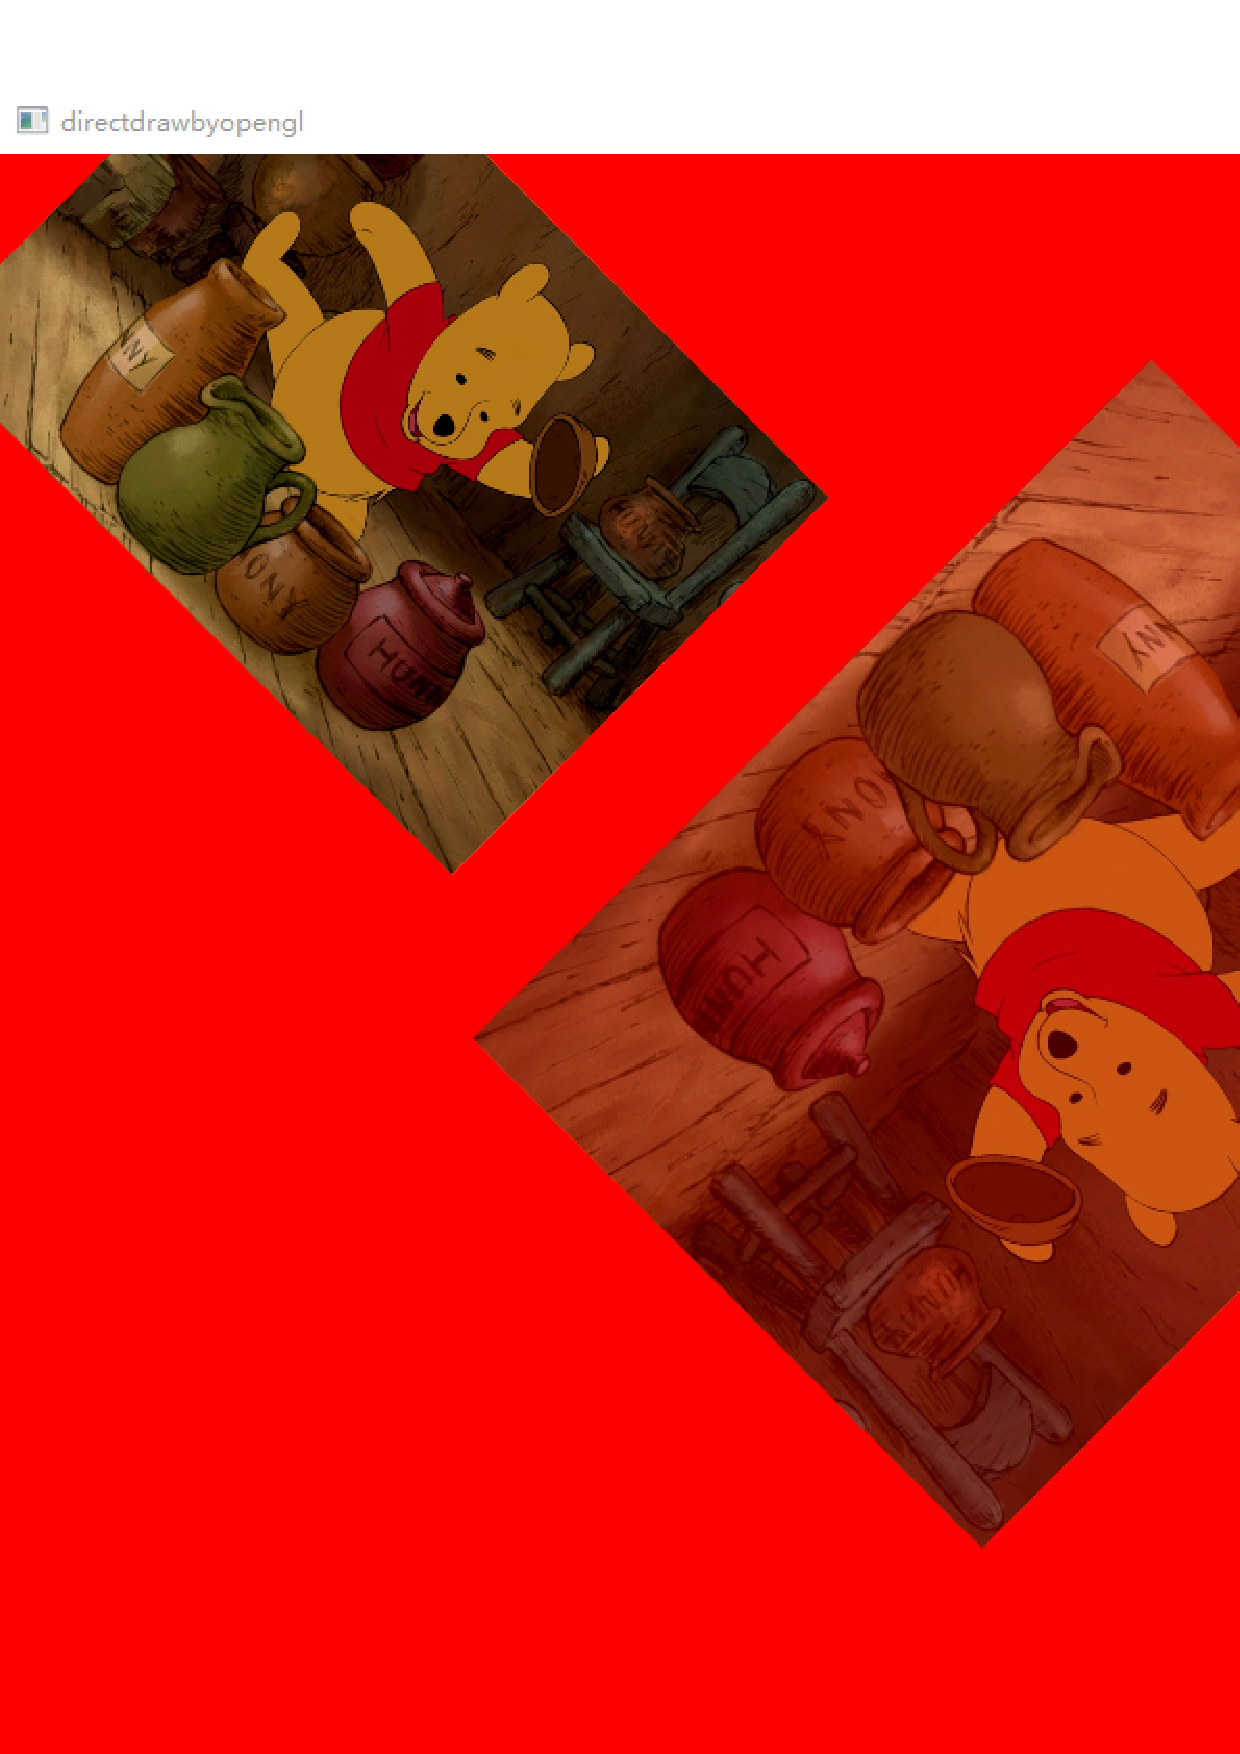
\includegraphics[width=0.95\textwidth]{the_book_image/p000011.pdf}} %图片路径
\caption{直接使用OpenGL绘制} %标题
\label{p000011} %索引
\end{figure}
%end图片


先来看看Qt Quick代码,
如\filesourcenumbernameone\ \ref{f000042}。

%\begin{spacing}{1.0}
\refstepcounter{filesourcenumber}\label{f000042}    %增加源代码编号
\FloatBarrier                                  %强制完成浮动体布局
\begin{thebookfilesourceone}[escapeinside={(*@}{@*)},
caption=GoodLuck,
title=\filesourcenumbernameone \thefilesourcenumber
]
/*directdrawbyopengl/main.qml*/
import QtQuick 2.9
import sstd.quick 1.0

Rectangle{
    id : root_object
    objectName: "root_object";
    width: 1024 ;
    height: 768 ;
    color: Qt.rgba(1,0,0,1);

    DrawImageItemRaw {

        width: parent.width /2  ;
        height: parent.height /2;
        anchors.centerIn: parent;
        transformOrigin: Item.Center ;
        rawImage : Qt.resolvedUrl( "0000.jpg" );

        Timer{
            repeat: true;
            running: true;
            interval : 500 ;
            triggeredOnStart: true;
            onTriggered: {
                parent.rotation += 15 ;
                if(parent.rotation>360){
                    parent.rotation -= 360 ;
                }
                parent.opacity = Math.random() * 0.3 + 0.7 ;
                parent.scale = Math.random() * 0.3 + 0.7   ;
            }
        }

    }


    Component.onCompleted : {
        Qt.createQmlObject(
"
import QtQuick 2.9
import sstd.quick 1.0

DrawImageItemRaw {
    width: 256   ;
    height: 256  ;
    anchors.top: parent.top                 ;
    anchors.right : parent.right            ;
    rawImage : Qt.resolvedUrl( '0000.jpg' ) ;
}

" , root_object  ) ;
    }

}/*Rectangle*/(*@\marginpar[\hfill\setlength\fboxsep{2pt}\fbox{\footnotesize{\kaishu\parbox{1em}{\setlength{\baselineskip}{2pt}\filesourcenumbernameone}}\footnotesize{\thefilesourcenumber}}]{\setlength\fboxsep{2pt}\fbox{\footnotesize{\kaishu\parbox{1em}{\setlength{\baselineskip}{2pt}\filesourcenumbernameone}}\footnotesize{\thefilesourcenumber}}}@*)\end{thebookfilesourceone}          %抄录环境
\addtocounter{lstlisting}{-1}   %sub lstlisting counter ...
%\end{spacing}


\begin{itemize}

\item 第3行引入自定义模块。
其对应的C{\sourcefonttwo{}+}{\sourcefonttwo{}+}代码如\filesourcenumbernameone\ \ref{f000043}:
%\begin{spacing}{1.0}
\refstepcounter{filesourcenumber}\label{f000043}    %增加源代码编号
\FloatBarrier                                  %强制完成浮动体布局
\begin{thebookfilesourceone}[escapeinside={(*@}{@*)},
caption=GoodLuck,
title=\filesourcenumbernameone \thefilesourcenumber
]
static inline void register_this() {
    qmlRegisterType<DrawImageItem>(
        "sstd.quick",
        1, 0,
        "DrawImageItemRaw");
}
Q_COREAPP_STARTUP_FUNCTION(register_this)(*@\marginpar[\hfill\setlength\fboxsep{2pt}\fbox{\footnotesize{\kaishu\parbox{1em}{\setlength{\baselineskip}{2pt}\filesourcenumbernameone}}\footnotesize{\thefilesourcenumber}}]{\setlength\fboxsep{2pt}\fbox{\footnotesize{\kaishu\parbox{1em}{\setlength{\baselineskip}{2pt}\filesourcenumbernameone}}\footnotesize{\thefilesourcenumber}}}@*)\end{thebookfilesourceone}          %抄录环境
\addtocounter{lstlisting}{-1}   %sub lstlisting counter ...
%\end{spacing}


本节的示例依然是静态加载,
实际上Qt Quick也支持以插件的形式动态加载组件。

\item 第12\raisebox{0.16ex}{\sourcefonttwo\~{}}35行演示了如何使用
自定义模块中的类“DrawImageItemRaw”。

使用C{\sourcefonttwo{}+}{\sourcefonttwo{}+}自定义的类与Qt Quick原生元素没有什么不同。
信号槽、平移、旋转、缩放……

不难发现,
使用Qt Quick可以将一切从极高的抽象层上
迅速的组装起来。

\item 第38\raisebox{0.16ex}{\sourcefonttwo\~{}}53行演示了直接在
Qt Quick里面编译Qt Quick源码并以此创建对象。

正如读者所见,
Qt Quick拥有脚本语言的所有特性,
并可以与Qt C{\sourcefonttwo{}+}{\sourcefonttwo{}+}无缝通信。

\end{itemize}

%\begin{spacing}{1.0}
\refstepcounter{filesourcenumber}\label{f000044}    %增加源代码编号
\FloatBarrier                                  %强制完成浮动体布局
\begin{thebookfilesourceone}[escapeinside={(*@}{@*)},
caption=GoodLuck,
title=\filesourcenumbernameone \thefilesourcenumber
]
/*directdrawbyopengl/main.cpp*/
#include <sstd_qt_and_qml_library.hpp>
#include "DrawImageItem.hpp"

int main(int argc, char ** argv) {

    /*初始化程序*/
    auto varApp = sstd_make_unique< sstd::Application >(argc, argv);
    /*初始化Qml/Quick引擎*/
    auto varWindow = sstd_make_unique< sstd::DefaultRoowWindow >();
    {
        /*获得Qml文件绝对路径*/
        auto varFullFileName = sstd::getLocalFileFullPath(
            QStringLiteral("myqml/directdrawbyopengl/main.qml"));

        /*加载Qml文件*/
        varWindow->load(varFullFileName);
        /*检查并报错*/
        if (varWindow->status() != sstd::LoadState::Ready) {
            qWarning() << QStringLiteral("can not load : ")
            << varFullFileName;
            return -1;
        }

    }

    varWindow->show();

    {
        /*运行时由C++端添加对象*/
        auto varRootObject = varWindow->getRootObject();
        assert(varRootObject);
        assert(varRootObject->objectName() == QStringLiteral("root_object"));
        auto varItem = sstd_new<DrawImageItem>();
        varItem->setParent(varRootObject);
        const auto varImage = QImage(sstd::getLocalFileFullFilePath(
            QStringLiteral("myqml/directdrawbyopengl/0000.jpg")));
        varItem->setImage(varImage);
        varItem->setWidth(360);
        varItem->setHeight(256);
        varItem->setTransformOrigin(QQuickItem::Center);
        varItem->setRotation(45);
        varItem->setParentItem(varRootObject);
    }

    {
        /*运行时由C++编译QML对象*/
        const auto varQmlCode = u8R"+++(

import QtQuick 2.9
import sstd.quick 1.0

DrawImageItemRaw {

    width: 256                             ;
    height: 256                            ;
    rawImage : Qt.resolvedUrl( "0000.jpg" );
    anchors.bottom: parent.bottom          ;
    anchors.right : parent.right           ;

}

)+++"sv;

        QQmlComponent varComponent{ varWindow->getEngine() };
        auto varContex = QQmlEngine::contextForObject( varWindow->getRootObject() );
        varComponent.setData(
            QByteArray( varQmlCode.data(),static_cast<int>(varQmlCode.size()) ),
            varContex->baseUrl()
        );
        auto varObject = sstd_runtime_cast<DrawImageItem>(
            varComponent.beginCreate( varContex ) );
        assert(varObject);
        varObject->setParent(varWindow->getRootObject());
        varObject->setParentItem(varWindow->getRootObject());
        varComponent.completeCreate();

    }

    return varApp->exec();

}(*@\marginpar[\hfill\setlength\fboxsep{2pt}\fbox{\footnotesize{\kaishu\parbox{1em}{\setlength{\baselineskip}{2pt}\filesourcenumbernameone}}\footnotesize{\thefilesourcenumber}}]{\setlength\fboxsep{2pt}\fbox{\footnotesize{\kaishu\parbox{1em}{\setlength{\baselineskip}{2pt}\filesourcenumbernameone}}\footnotesize{\thefilesourcenumber}}}@*)\end{thebookfilesourceone}          %抄录环境
\addtocounter{lstlisting}{-1}   %sub lstlisting counter ...
%\end{spacing}









%使用XeLaTeX编译
%版权所有,翻版必究
%本文件由程序自动生成,任何修改将被覆盖
%2019 年 01 月 23 日










% ______all_key_words
% the_book_chapter the_book_subsection the_book_subsubsection
% the_book_section the_book_image the_book_table
% the_book_file the_book_tree_file the_book_command_file
% littlelongworld tabbing ref
% figurename tablename filesourcenumbernameone
% treeindexnumbernameone commandnumbernameone footnote
% item itemize comment textbullet
% \hspace*{\parindent}







%使用XeLaTeX编译
%版权所有,翻版必究
%本文件由程序自动生成,任何修改将被覆盖
%2019 年 01 月 23 日



